\section{辐射场重构方法影响因素研究}
本研究分别对简单空间单源辐射场、简单空间多源辐射场、带有屏蔽空间单源辐射场、带有屏蔽空间多源辐射场分别进行Geant4模拟,下面分别将源项数量、辐射场空间状况以及测量点数据为因变量,测评本论文提出的辐射场重构方法效果。

Geant4模拟主要分为初始化和运行:初始化为模拟的参数进行定义,包括1)定义几何体2)设置物理过程3)定义发射粒子;运行为Geant4代码执行时,Geant4内核所执行的具体内容,包括1)导入几何体结构2)循环执行Event(Event为Geant4中粒子发射)。其中,对于不同辐射场的初始化,本研究都设置相同的物理过程,即仅考虑电磁相互作用,电磁相互作用主要包含以下物理过程:光电效应、康普顿效应、电子对效应、韧致辐射、瑞利散射等。对于Geant4的几何体定义和粒子源设置,在下面不同影响因素研究中分别进行介绍。

\subsection{源项数量对辐射场重构效果的影响}
为探究源项数量对辐射场重构效果的影响,本论文分别对单源和多源情况分别进行Geant4模拟。

对于简单空间单源辐射场,整体辐射场空间设置为$ 3m \times 4m \times 5m $的立方体三维空间,辐射场材料设置为空气,几何体仅设置$ 50mm \times 50mm \times 50mm $的CsI材料进行探测,粒子源设置为能量为$0.662MeV$的$ ^{137}Cs $点源,点源位置设置在空间几何中心。对于简单空间多源辐射场,几何体也仅设置$ 50mm \times 50mm \times 50mm $的CsI材料,粒子源设置将分别定义三个位置不同的点源,分别为能量为$ 0.662MeV $的$ ^{137}Cs $点源,位置设为$ (-1.03m, -1.38m, -2.02m) $;能量为$ 0.835MeV $的$ ^{54}Mn $点源,位置设在$ (-1.03m, 1.57m, -1.72m) $以及能量为$ 0.662MeV $的$ ^{137}Cs $点源,位置设为$ (0.93m, 0.57m, 1.32m) $。Geant4模拟可视化效果如图\ref{Geant4模拟单源辐射场和多源辐射场}所示。

\begin{figure}[htbp]
    \subfigure[单放射源无屏蔽空间]{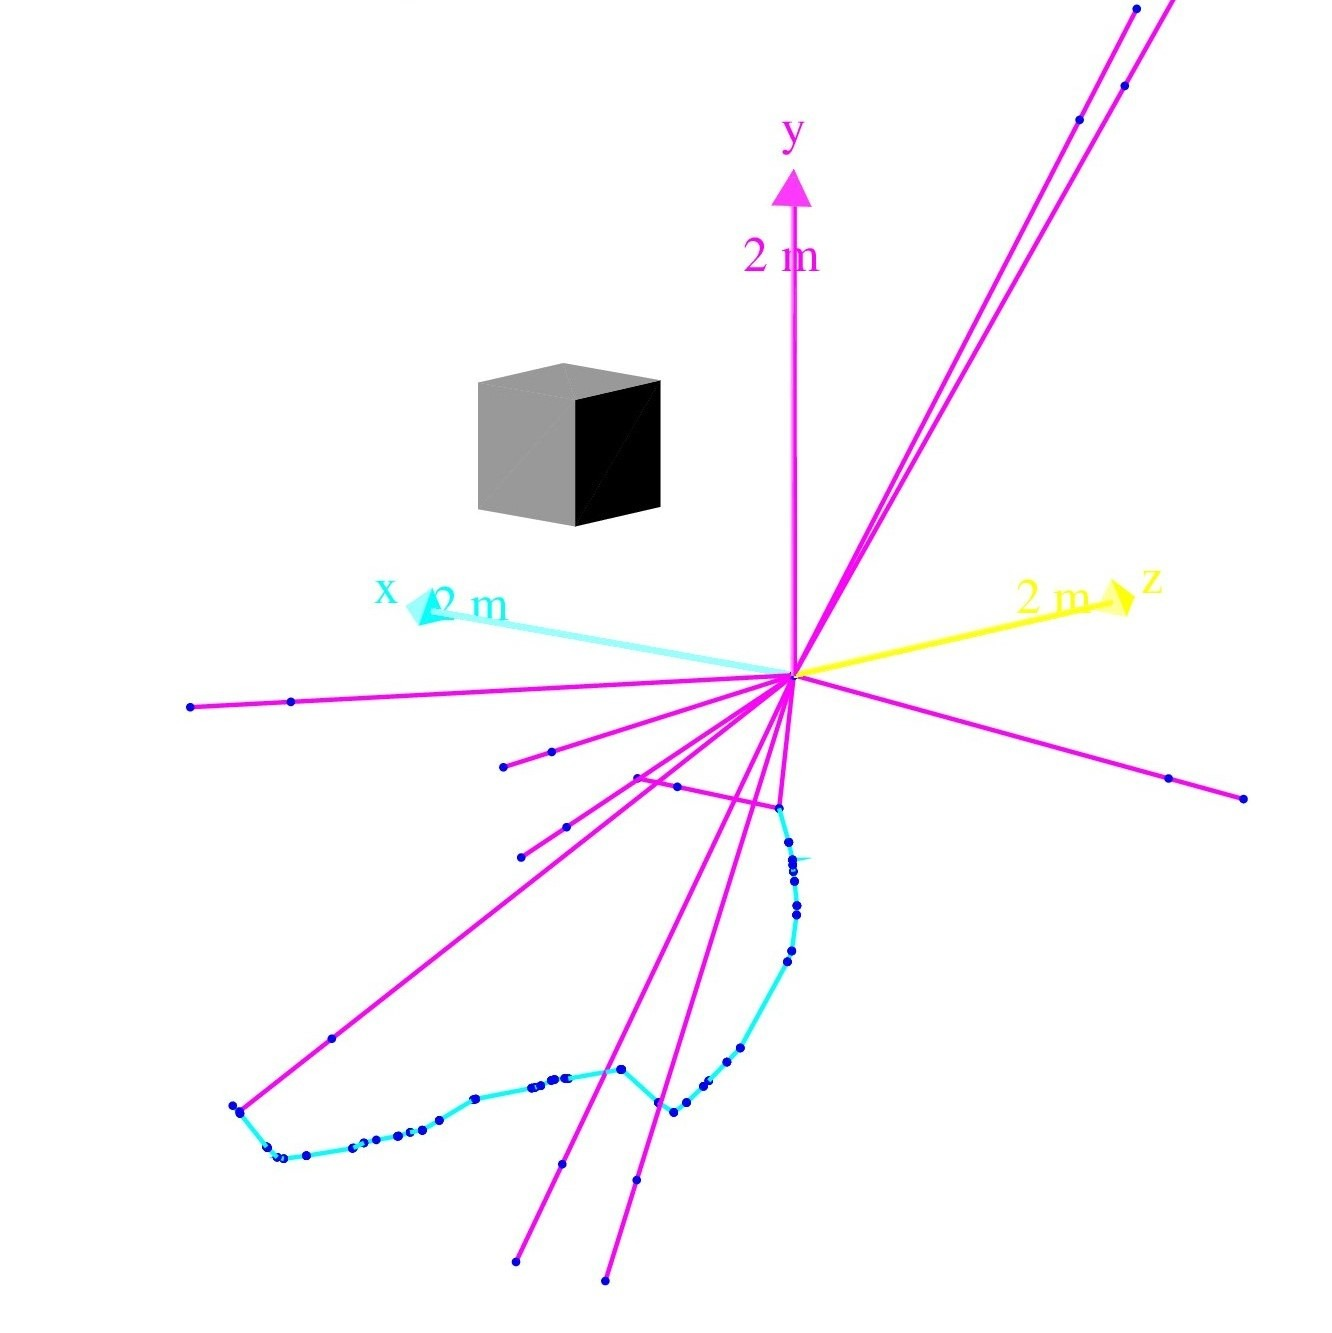
\includegraphics[width=0.45\textwidth]{figures/SingleSource.jpg}\label{fig:exph1}}
    \subfigure[多放射源无屏蔽空间]{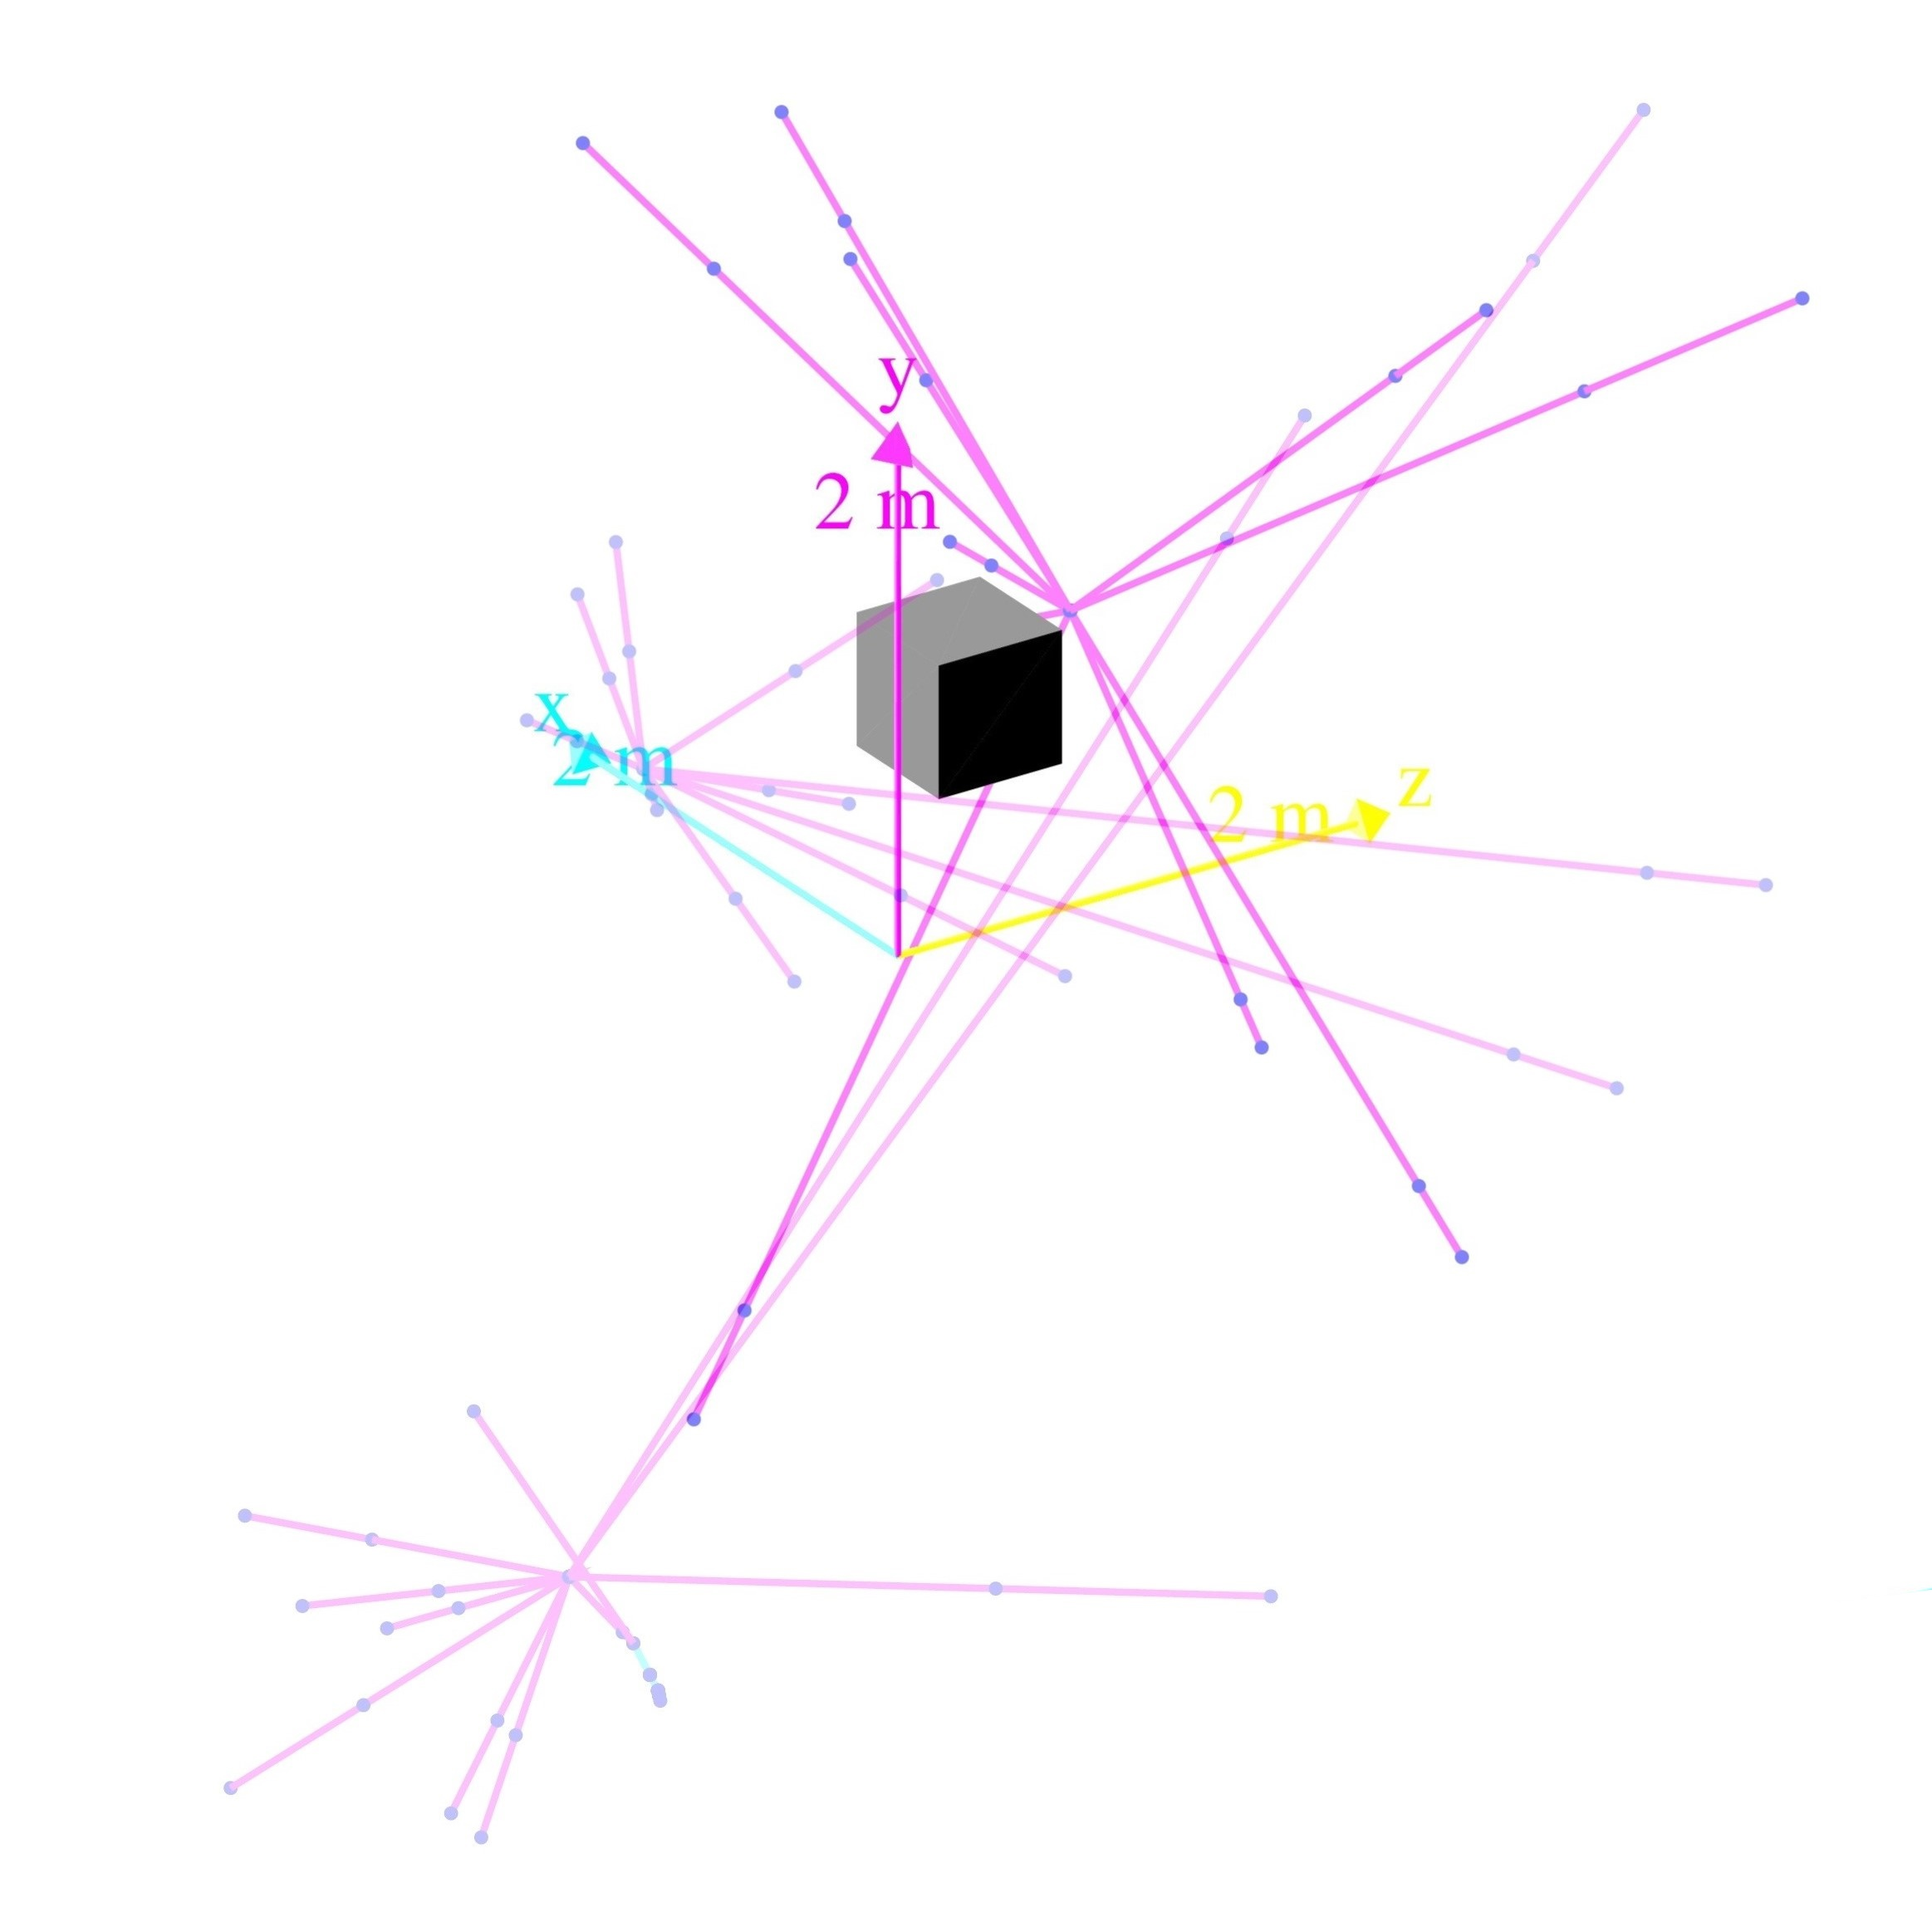
\includegraphics[width=0.45\textwidth]{figures/MultiSources.jpg}\label{fig:exgr1}}
    \caption{Geant4模拟单源辐射场和多源辐射场}
    \label{Geant4模拟单源辐射场和多源辐射场}
\end{figure}

通过Geant4框架分别对单源无屏蔽辐射场和多源无屏蔽辐射场进行模拟仿真,获得空间辐射场数据使用ROOT绘制,如图\ref{Geant4模拟单源辐射场和多源辐射场的剂量分布}所示。

\begin{figure}[htbp]
    \subfigure[单放射源无屏蔽辐射场剂量分布]{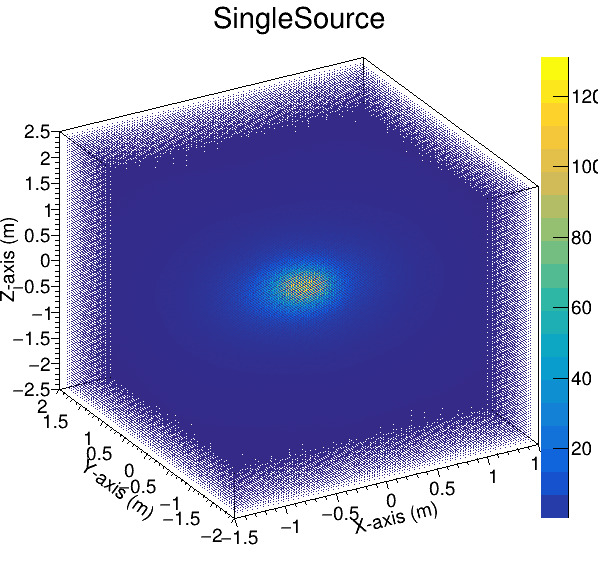
\includegraphics[width=0.45\textwidth]{figures/SingleSource.png}\label{fig:exph2}}
    \subfigure[多放射源无屏蔽辐射场剂量分布]{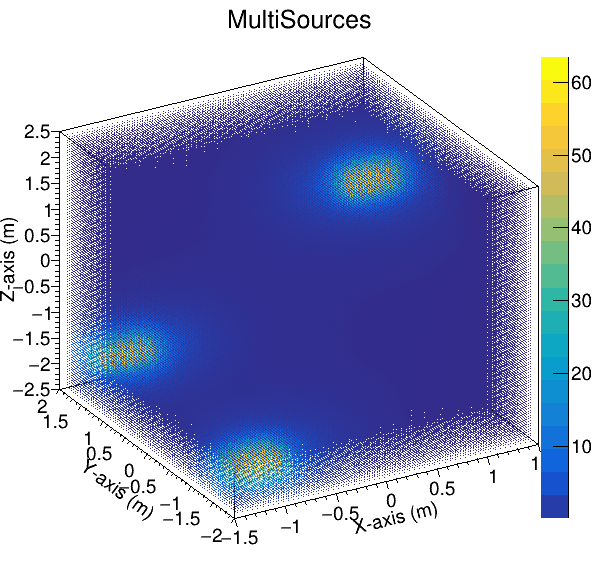
\includegraphics[width=0.45\textwidth]{figures/MultiSources.png}\label{fig:exgr2}}
    \caption{Geant4模拟单源辐射场和多源辐射场的剂量分布}
    \label{Geant4模拟单源辐射场和多源辐射场的剂量分布}
\end{figure}

从上图可以看出,在无屏蔽的情况下,辐射场剂量分布与源项数量相关。由于Geant4没有模拟天然本底,并且$ \gamma $射线在空气中有一定衰减,因此在各个源项相距较远的情况下,$ \gamma $辐射场剂量率分布源项越多,多源辐射场剂量分布可以看作为多个单源辐射场剂量分布加和。

根据Geant4重构出的辐射场,先每隔$ 50cm $测量一个数据量,共测量$ 6 \times 8 \times 10 $个数据点,对辐射场进行插值重构,再根据辐射场重构方法选取若干测量点数据,最终得到重构辐射场数据。将重构出的插值数据与Geant4模拟仿真的辐射场剂量率相比,得到不同源项数量与重构片插值的结果如:

\begin{table}[htbp]
    \centering
    \caption{\label{tab:test1}不同源项数量下重构插值方法对辐射场剂量率的相对偏差}
    \begin{tabular}{lcc}
        \toprule
        插值坐标(m)              & 单源辐射场相对偏差(\%) & 多源辐射场相对偏差(\%) \\
        \midrule
        $ (-1.25,-1.75,-2.45) $  & 38.29                  & 61.43                  \\
        $ (-1.25,-0.75,-0.65) $  & 2.43                   & 6.78                   \\
        $ (-0.85,-1.35,0.35) $   & 0.22                   & 3.05                   \\
        $ (-0.65,-0.75,0.15) $   & 7.25                   & 0.75                   \\
        $ (-0.25,-0.75,-0.45) $  & 1.72                   & 3.01                   \\
        $ (-0.25,-0.15,0.55) $   & 6.98                   & 2.05                   \\
        $ (0.35,-1.55,0.15) $    & 2.76                   & 1.42                   \\
        $ (-1.25,1.05,1.95) $    & 3.47                   & 0.01                   \\
        $ (0.75,0.85,1.35) $     & 0.10                   & 31.37                  \\
        辐射场平均相对偏差绝对值 & 6.15                   & 13.4                   \\
        \bottomrule
    \end{tabular}
    \label{不同源项数量下重构插值方法对辐射场剂量率的相对偏差}
\end{table}

表\ref{不同源项数量下重构插值方法对辐射场剂量率的相对偏差}列举了部分插值点和辐射场整体插值点相对偏差。从整体偏差值数据可以看出,单源辐射场重构整体相对偏差小于多源辐射场重构整体相对偏差。从辐射场插值点相对偏差值可以看出,离测量点越近的重构点,与Geant4模拟值的偏差越小;在辐射场空间边缘和源项附近,插值重构相对偏差较大。在空间边缘辐射场偏差较大的原因是Geant4模拟辐射场剂量值较低,导致重构相对偏差较大;源项附近插值相对偏差较大的原因为插值算法对梯度较大的领域重构效果不够好。

\subsection{空间状况对辐射场重构效果的影响}
为探究空间状况对辐射场重构效果的影响,本论文分别对无屏蔽空间和带有屏蔽空间情况分别进行Geant4模拟。

对于无屏蔽空间辐射场,整体辐射场空间设置为$ 3m \times 4m \times 5m $的立方体三维空间,辐射场材料设定为空气;探测几何体设置为$ 50mm \times 50mm \times 50mm $的$ CsI $材料,不设置屏蔽物;粒子源设置为能量为$ 0.662MeV $的$ ^{137}Cs $点源,点源位置设置为辐射场空间几何中心。对于有屏蔽空间辐射场,探测几何同样设置为$ 50mm \times 50mm \times 50mm $的$ CsI $材料,设置两个屏蔽物:一个设置为$ 2m \times 1m \times 0.02m $铅板,位置设为$ (0.4m, 0.8m, 1.7m) $;另一个屏蔽物设置为$ 2.5m \times 1.8m \times 0.3m $的钢筋混凝土材料,位置设为$ (0.6m, -0.6m, -1.25m) $;粒子源设置为能量为$ 0.662MeV $的$ ^{137}Cs $点源,点源位置设置为辐射场空间几何中心。Geant4模拟可视化效果如图\ref{Geant4模拟无屏蔽空间辐射场和有屏蔽空间辐射场}所示。

\begin{figure}[htbp]
    \subfigure[单放射源无屏蔽空间]{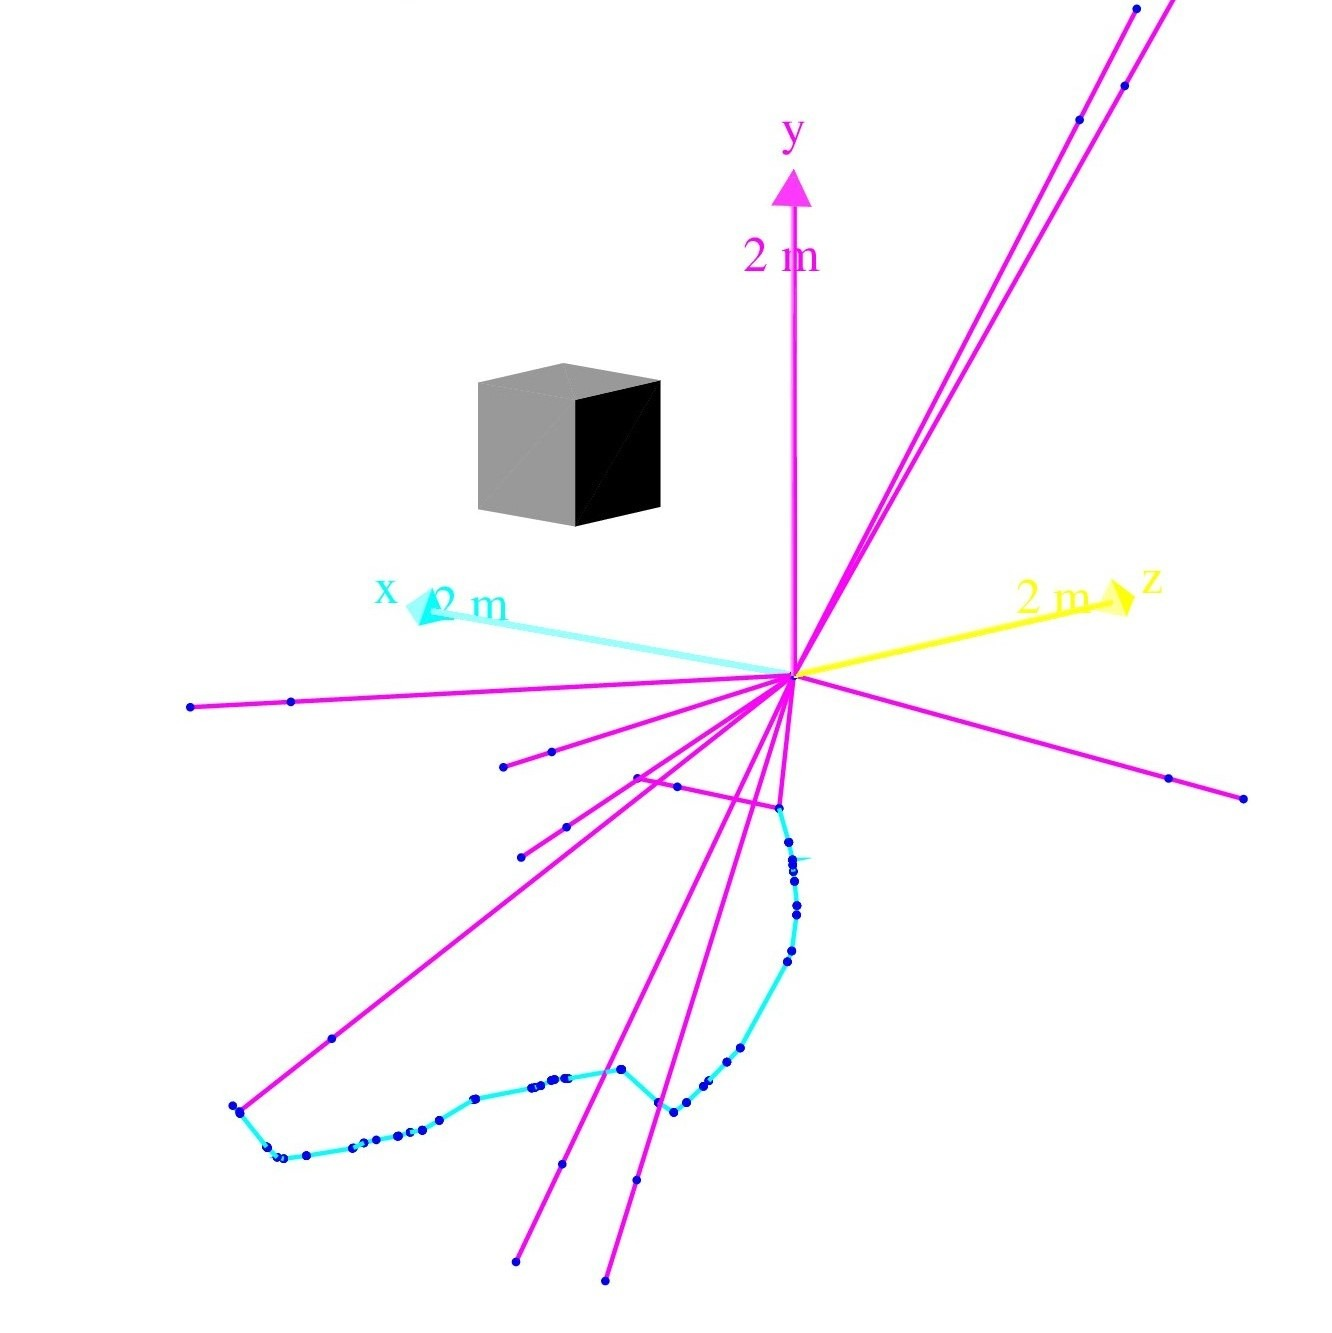
\includegraphics[width=0.45\textwidth]{figures/SingleSource.jpg}\label{fig:exph3}}
    \subfigure[单放射源有屏蔽空间]{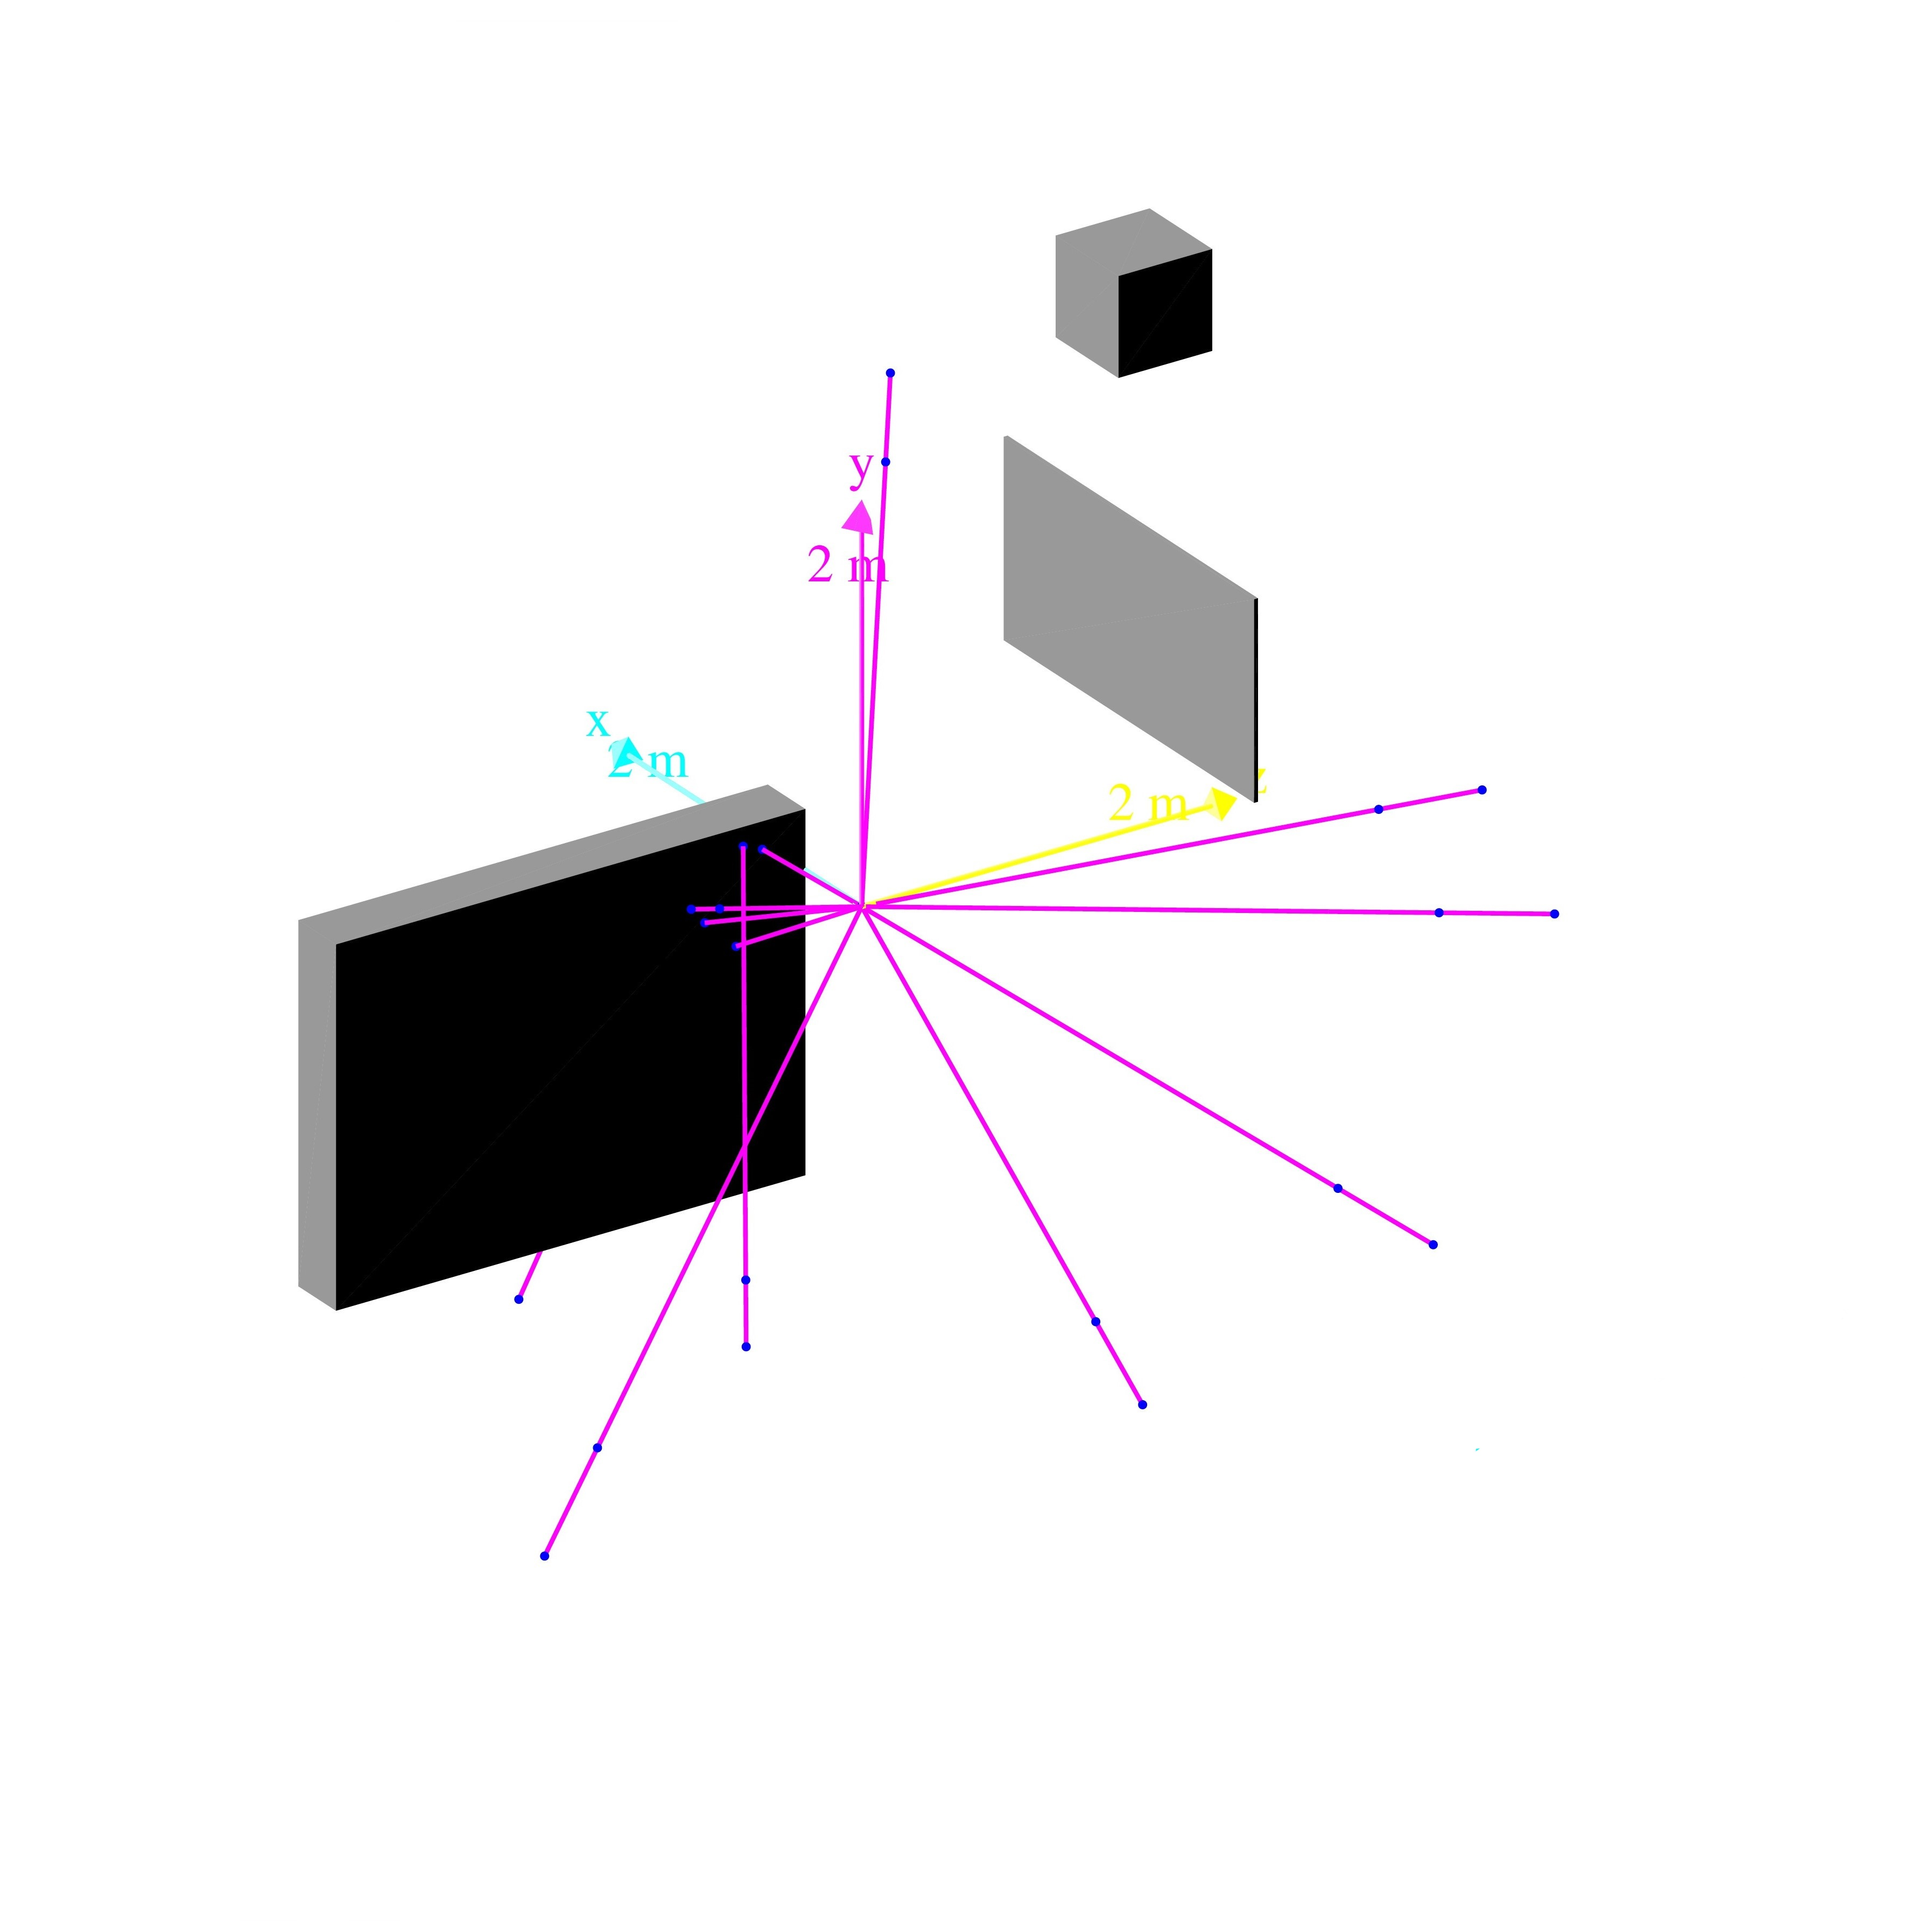
\includegraphics[width=0.45\textwidth]{figures/SingleSourceShield.jpg}\label{fig:exgr3}}
    \caption{Geant4模拟无屏蔽空间辐射场和有屏蔽空间辐射场}
    \label{Geant4模拟无屏蔽空间辐射场和有屏蔽空间辐射场}
\end{figure}

通过Geant4框架分别对单点源无屏蔽辐射场和单点源带有屏蔽辐射场进行模拟仿真,获得空间辐射场数据使用ROOT绘制,如图\ref{Geant4模拟无屏蔽辐射场和有屏蔽辐射场的剂量分布}所示。

\begin{figure}[htbp]
    \subfigure[单点源无屏蔽辐射场剂量分布]{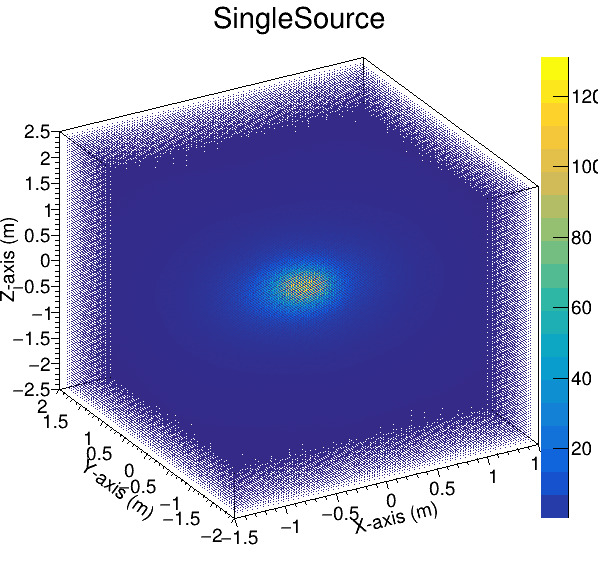
\includegraphics[width=0.45\textwidth]{figures/SingleSource.png}\label{fig:exph4}}
    \subfigure[单点源有屏蔽辐射场剂量分布]{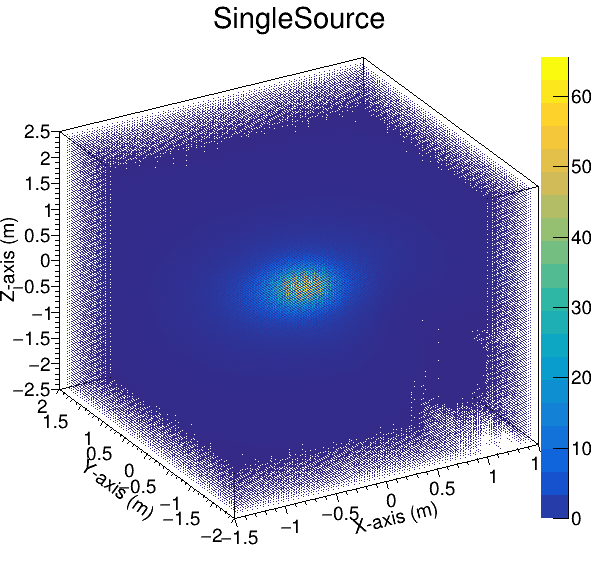
\includegraphics[width=0.45\textwidth]{figures/SingleSoourceShielded.png}\label{fig:exgr4}}
    \caption{Geant4模拟单点源无屏蔽辐射场和单点源有屏蔽辐射场的剂量分布}
    \label{Geant4模拟无屏蔽辐射场和有屏蔽辐射场的剂量分布}
\end{figure}

从图\ref{Geant4模拟无屏蔽辐射场和有屏蔽辐射场的剂量分布}中可以看出,在单点源情况下,辐射场剂量分布与空间状况相关。在屏蔽物周围的领域内,辐射场剂量变化梯度较大,且梯度大小与屏蔽物材料有关,屏蔽材料的线衰减系数越大,辐射场剂量变化梯度越大。

根据Geant4重构出的辐射场,先每隔$ 50cm $测量一个数据量,共测量$ 6 \times 8 \times 10 $个数据点,对辐射场进行插值重构,再根据辐射场重构方法选取若干测量点数据,最终得到重构辐射场数据。将重构出的插值数据与Geant4模拟仿真的辐射场剂量率相比,得到不同源项数量与重构片插值的结果如:

\begin{table}[htbp]
    \centering
    \caption{\label{tab:test2}不同空间状况下重构插值方法对辐射场剂量率的相对偏差}
    \begin{tabular}{lcc}
        \toprule
        插值坐标(m)              & 无屏蔽辐射场相对偏差(\%) & 有屏蔽辐射场相对偏差(\%) \\
        \midrule
        $ (-1.25,-1.75,-2.45) $  & 38.29                    & 2.43                     \\
        $ (-1.25,-0.75,-0.65) $  & 2.43                     & 3.48                     \\
        $ (-0.85,-1.35,0.35) $   & 0.22                     & 6.03                     \\
        $ (-0.65,-0.75,0.15) $   & 7.25                     & 44.89                    \\
        $ (-0.25,-0.75,-0.45) $  & 1.72                     & 59.07                    \\
        $ (-0.25,-0.15,0.55) $   & 6.98                     & 16.57                    \\
        $ (0.35,-1.55,0.15) $    & 2.76                     & 2.19                     \\
        $ (-1.25,1.05,1.95) $    & 3.47                     & 3.21                     \\
        $ (0.75,0.85,1.35) $     & 0.10                     & 0.85                     \\
        辐射场平均相对偏差绝对值 & 6.15                     & 53.46                    \\
        \bottomrule
    \end{tabular}
    \label{不同空间状况下重构插值方法对辐射场剂量率的相对偏差}
\end{table}

% //对无屏蔽空间辐射场插值重构相对偏差与带有屏蔽空间辐射场插值重构相对偏差进行分析,可以与上面源项数量数据相对比!
表\ref{不同空间状况下重构插值方法对辐射场剂量率的相对偏差}列举了部分插值点和辐射场整体插值点相对偏差。从整体偏差值数据可以看出,无屏蔽辐射场重构整体相对偏差小于带有屏蔽辐射场重构的整体相对偏差。从带有屏蔽的辐射场插值点相对偏差中可以看出,在靠近屏蔽物的地方,插值重构效果不是很好,说明插值重构在变化梯度大的位置重构的效果不够优秀。将空间状况与辐射场相对偏差数据同源项数量与相对偏差数据相比,可以看出空间状况对辐射场重构效果影响更大,或者说,本论文提出的辐射场重构方法对带有屏蔽的辐射场重构效果相对较差。

\subsection{测量点数据对辐射场重构效果影响}
为探究测量点数据对辐射场重构效果的影响,本论文分别对单点源无屏蔽空间辐射场、多点源无屏蔽空间辐射场、单点源带屏蔽空间辐射场、多点源带屏蔽空间辐射场四种Geant4模拟辐射场进行不同测量点数量、测量点位置对比、分析。

对于以上四种不同类型辐射场,初始测点数量均为$ 6 \times 8 \times 10 $个,根据本论文提出的辐射场插值重构方法,对于单点源无屏蔽辐射场最终测点数量为$ 480 $个;多点源无屏蔽辐射场最终测点数量为$ 489 $个;单点源有屏蔽辐射场最终测点数量为$ 491 $个;多点源有屏蔽辐射场最终测量点数量为$ 483 $个。四种辐射场相对偏差值大小及分布如图\ref{空间辐射场插值重构相对偏差分布}所示。

\begin{figure}[htbp]
    \centering
    \subfigure[单点源无屏蔽空间场]{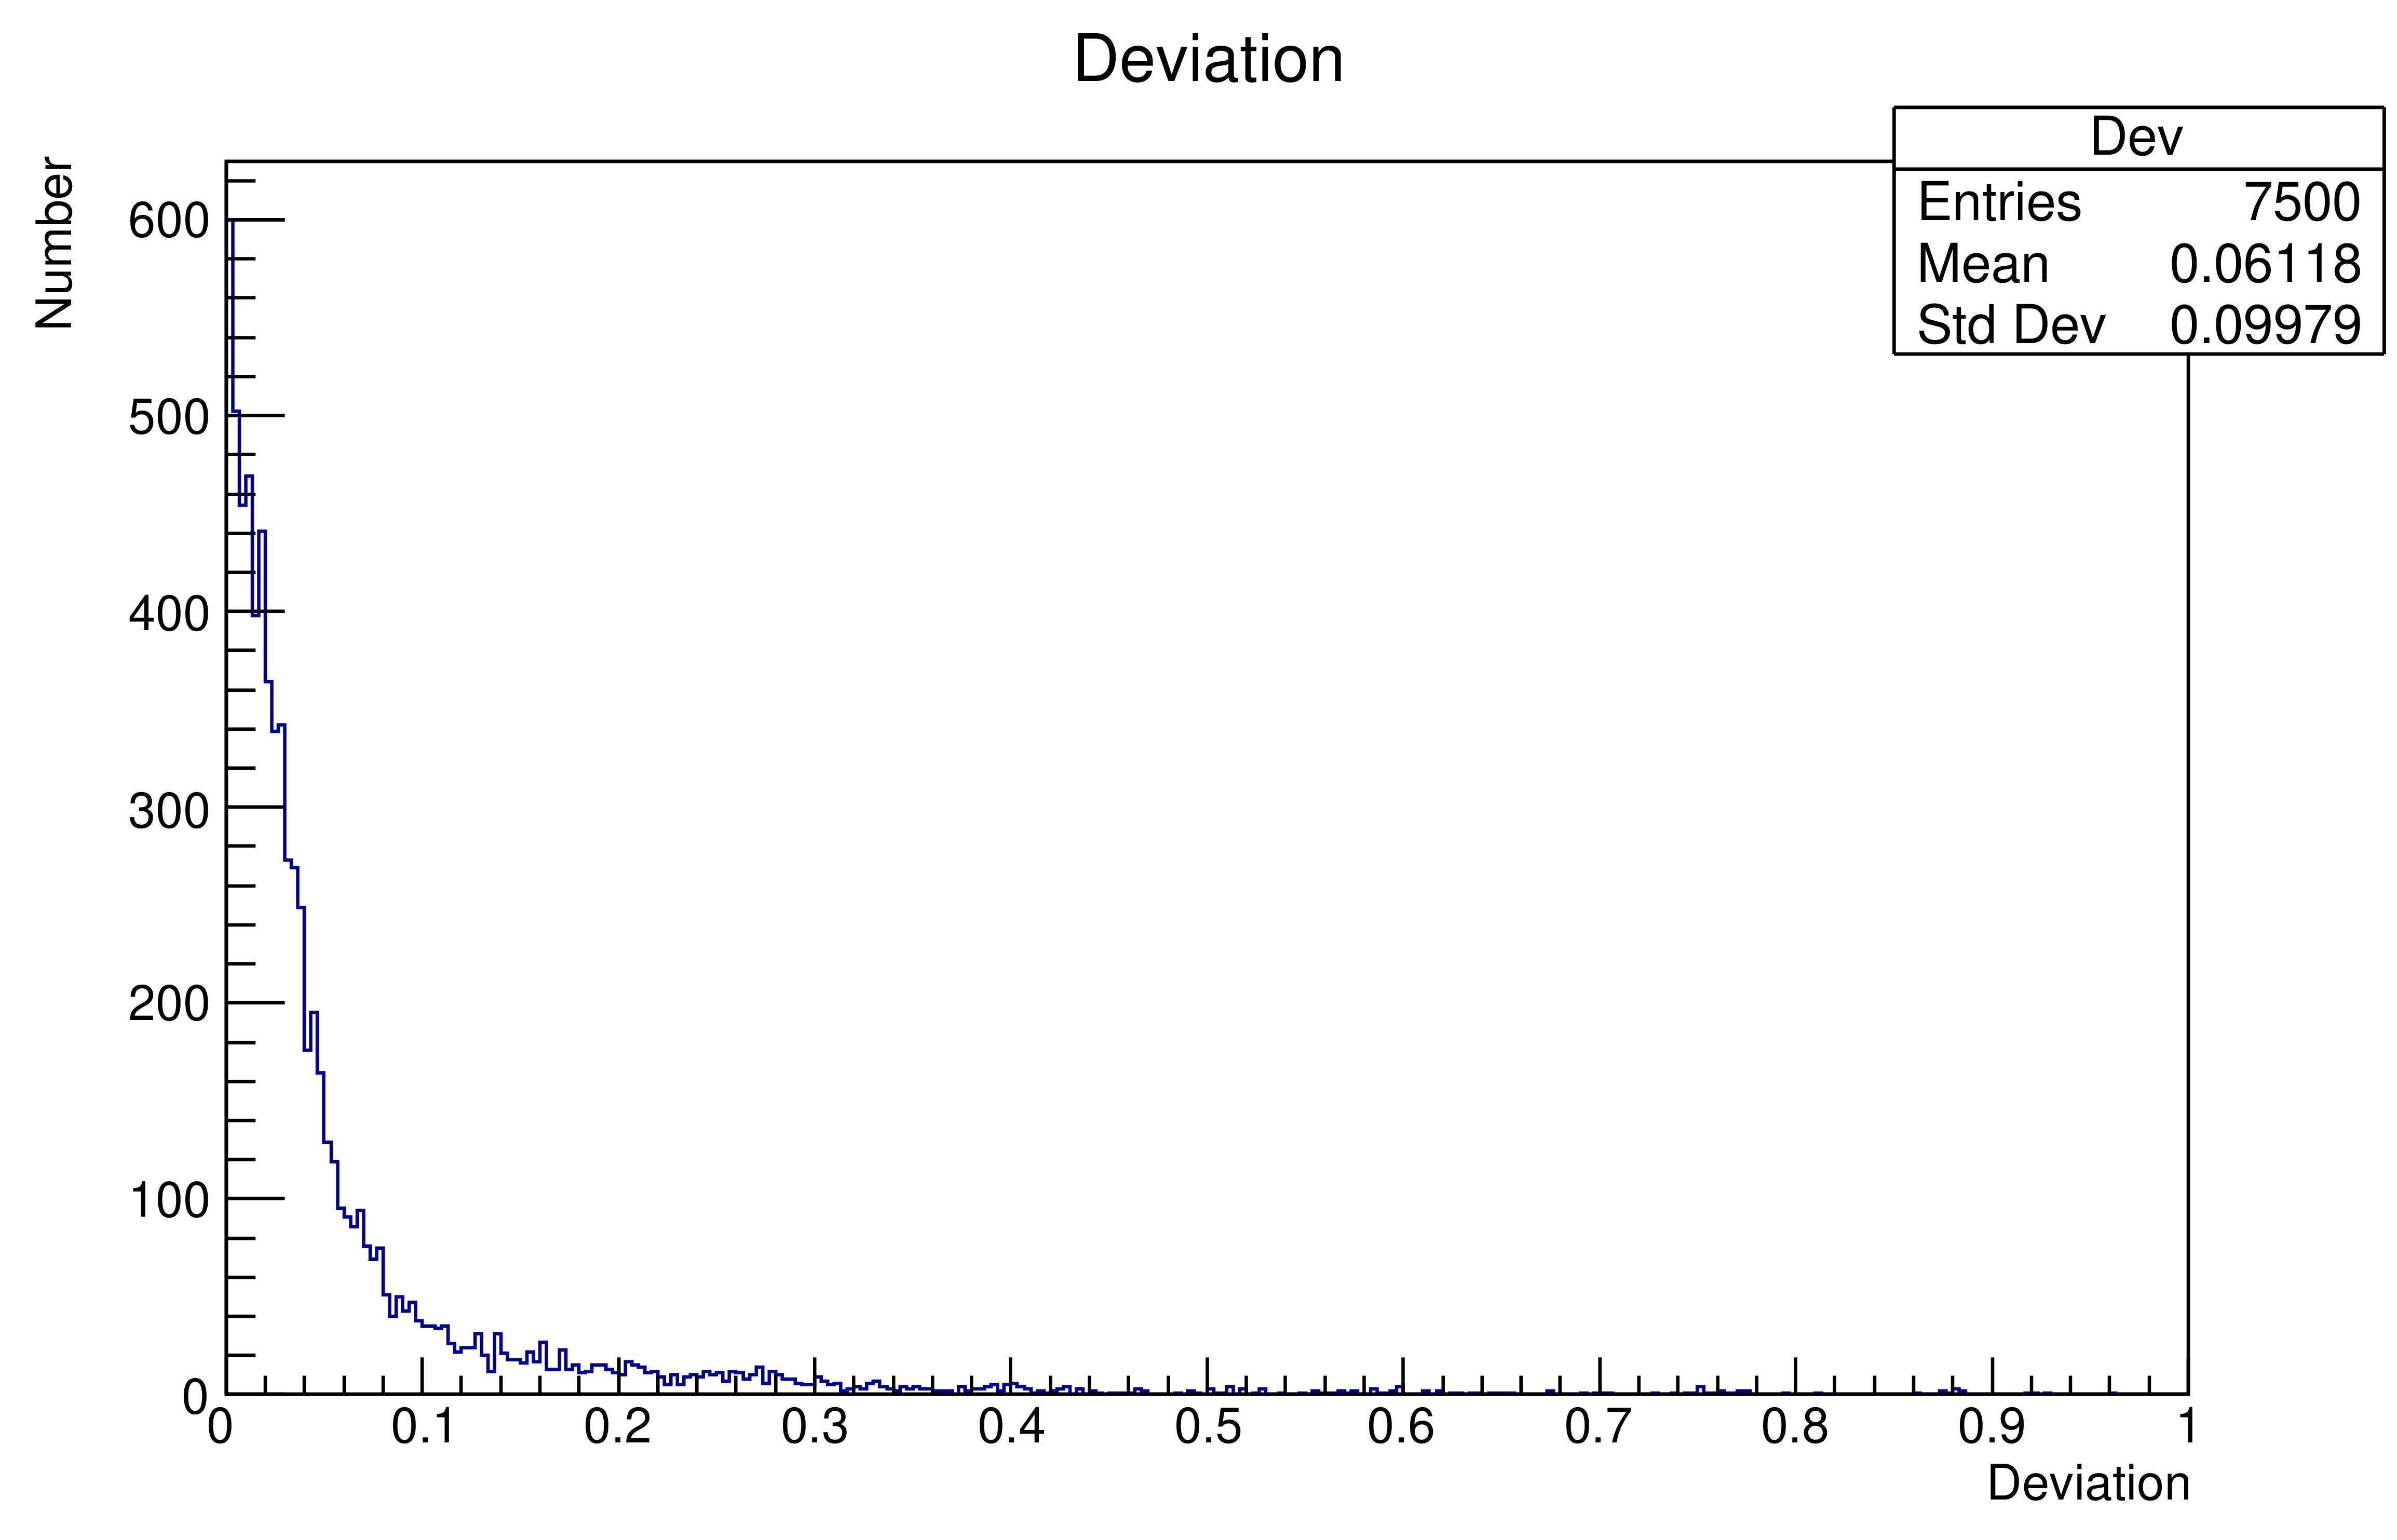
\includegraphics[width=0.45\textwidth]{figures/Deviation/SingleSourceUnshield.jpg}\label{fig:exph5}}
    \subfigure[多点源无屏蔽空间场]{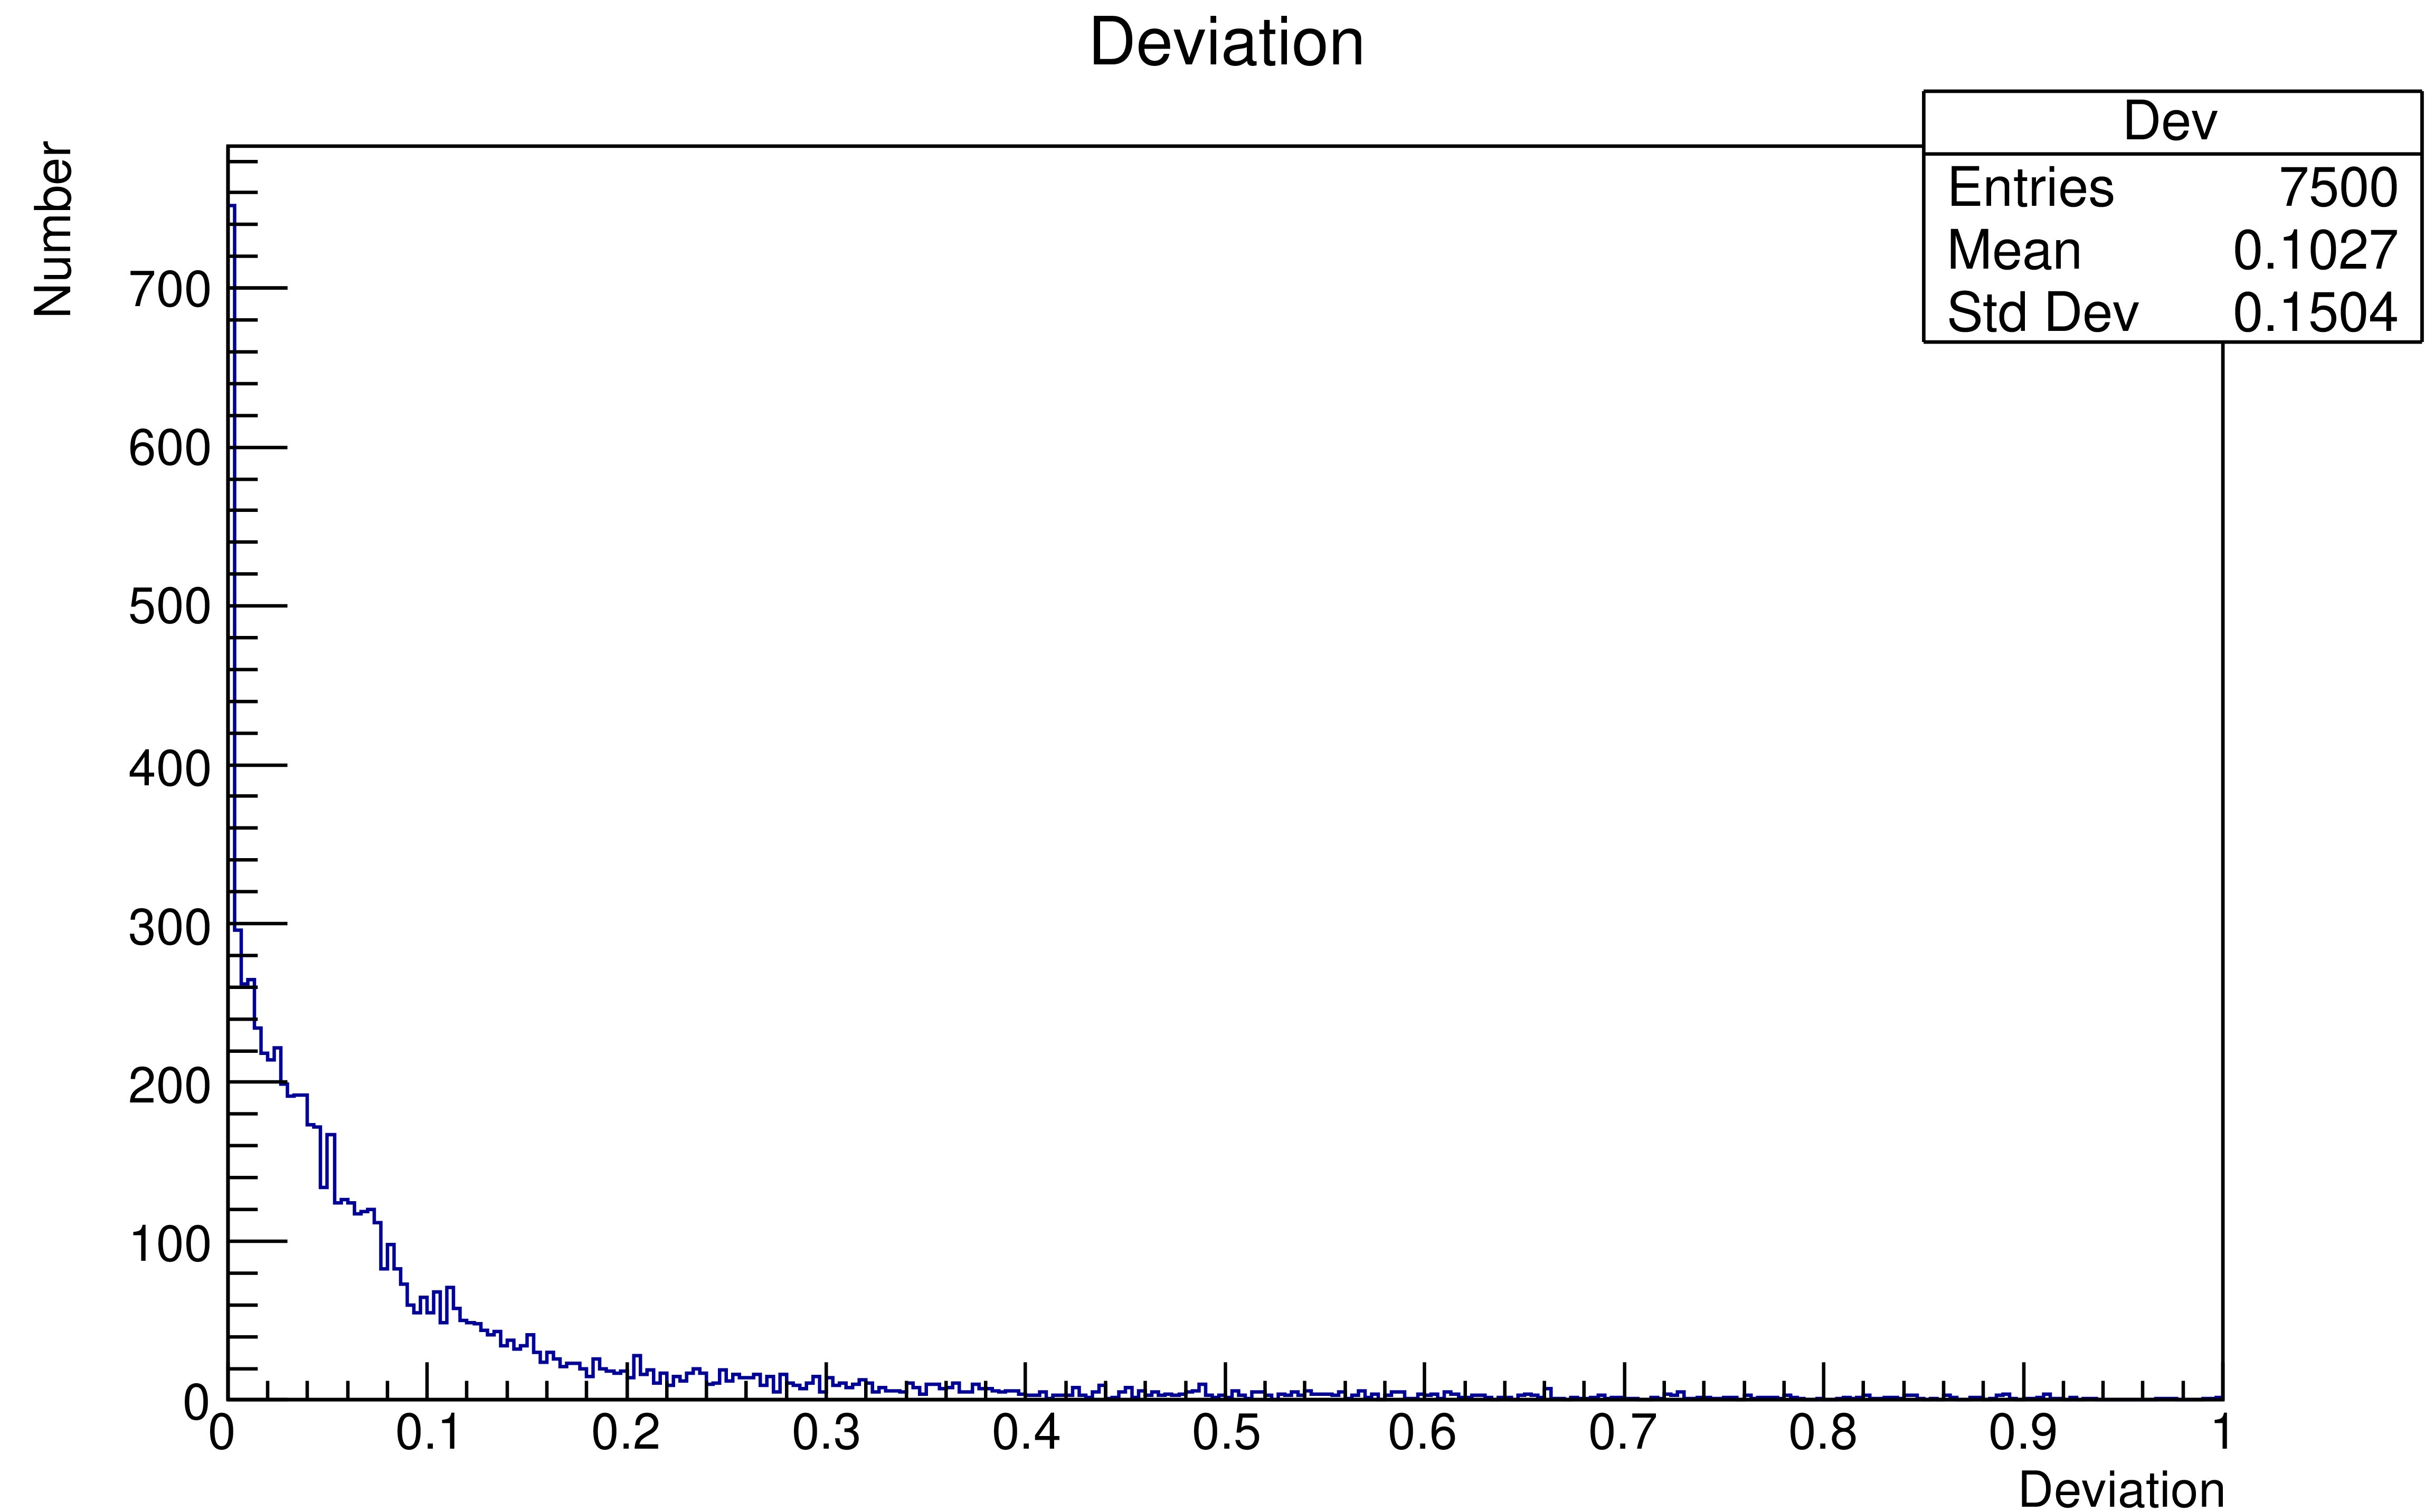
\includegraphics[width=0.45\textwidth]{figures/Deviation/MultiSourcesUnshield.jpg}\label{fig:exgr5}}

    \subfigure[单点源无屏蔽空间场]{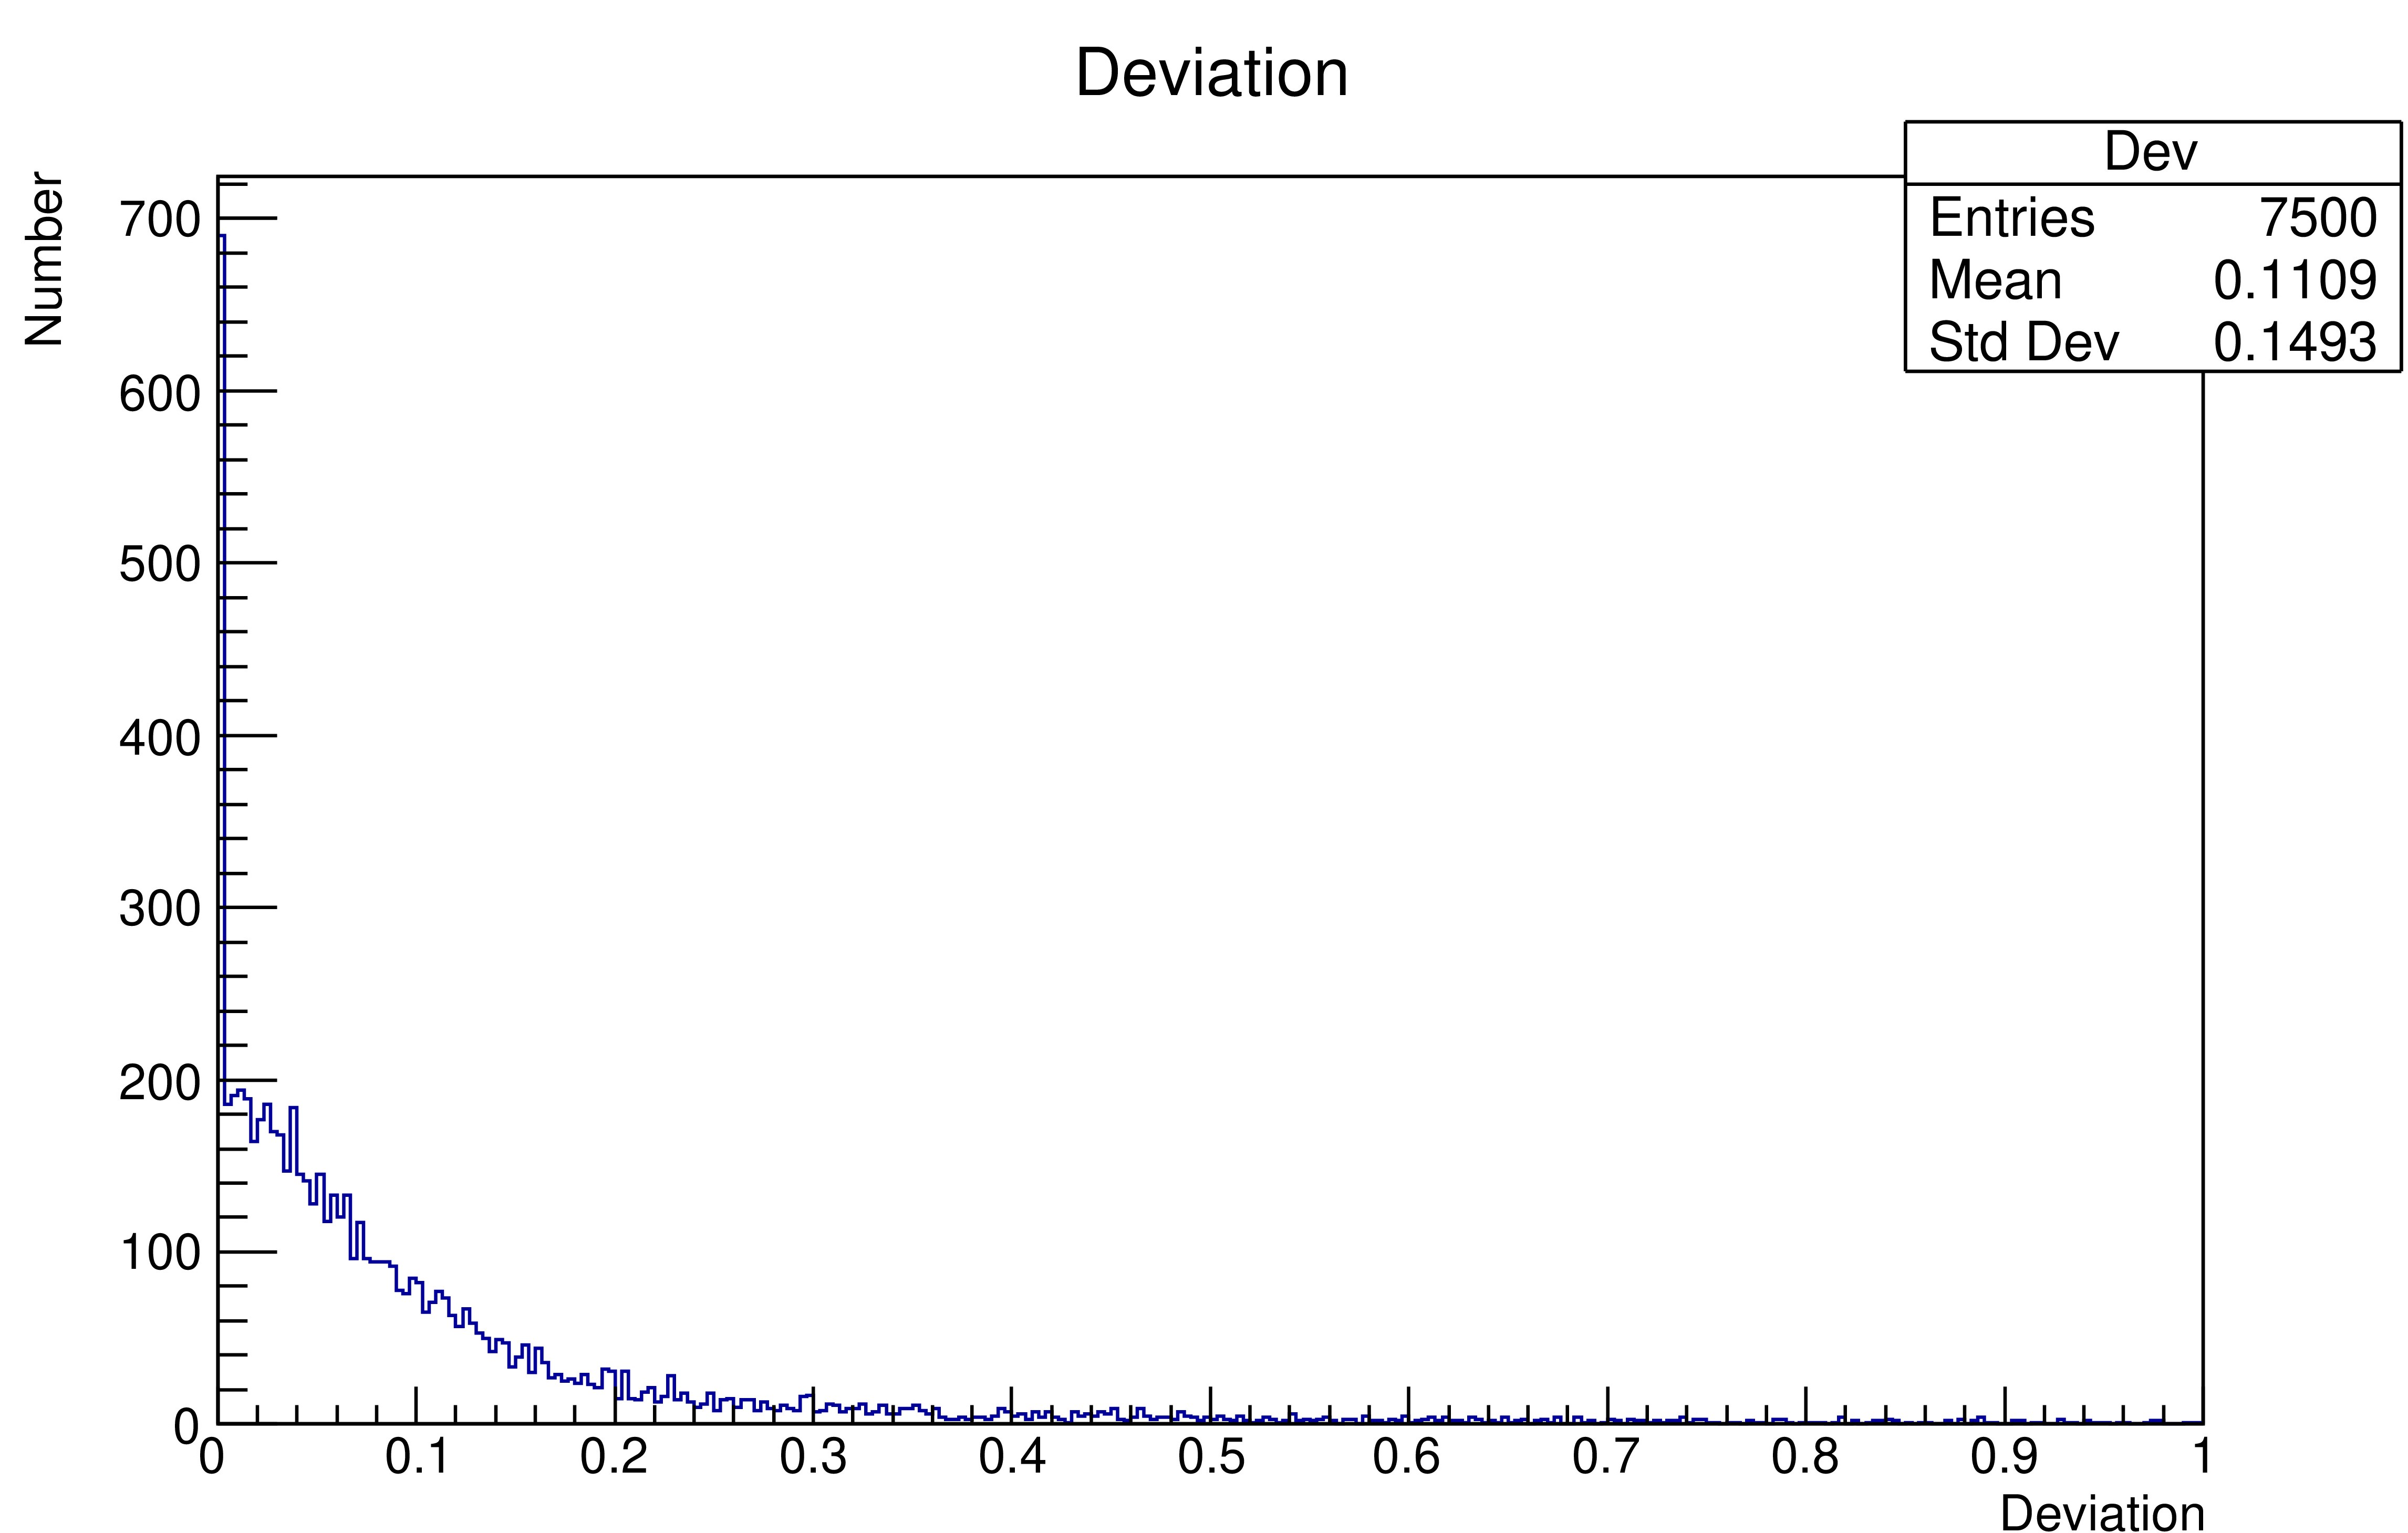
\includegraphics[width=0.45\textwidth]{figures/Deviation/SingleSourceShield.jpg}\label{fig:exph6}}
    \subfigure[多点源有屏蔽空间场]{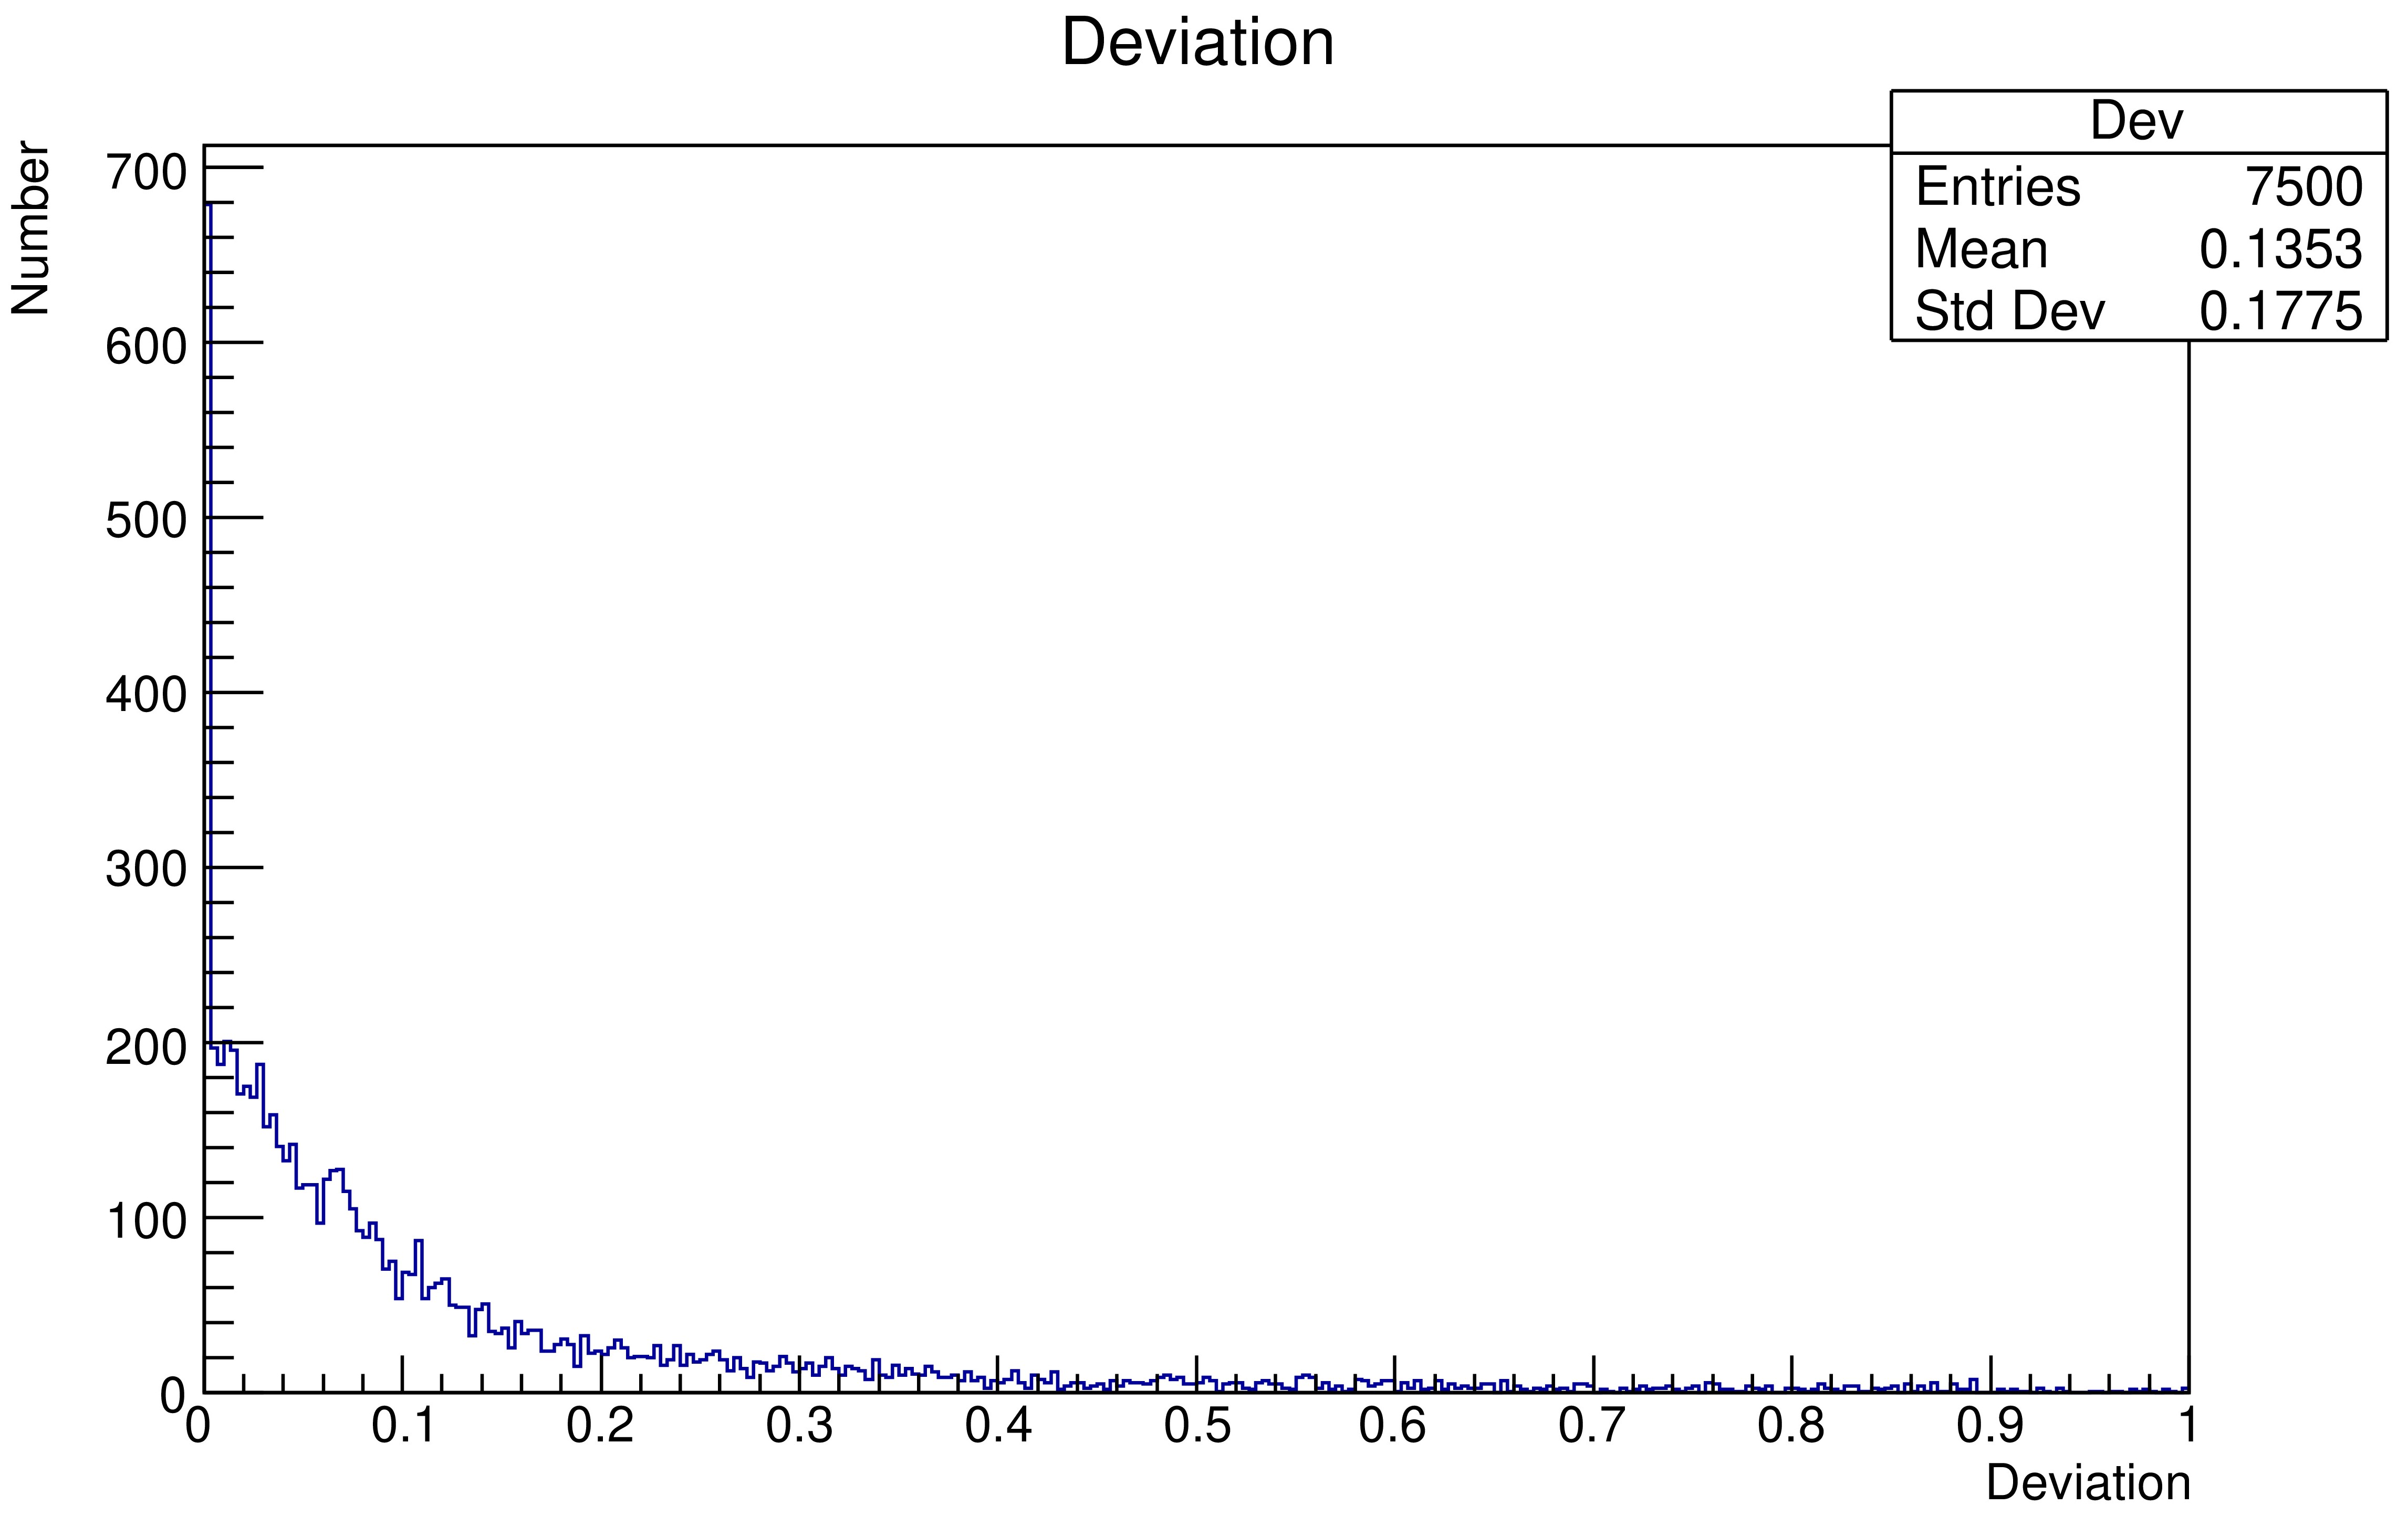
\includegraphics[width=0.45\textwidth]{figures/Deviation/MultiSourcesShield.jpg}\label{fig:exgr6}}

    \caption{空间辐射场插值重构相对偏差分布}
    \label{空间辐射场插值重构相对偏差分布}
\end{figure}

从辐射场重构相对偏差分布中可以看出,相对偏差大小从低到高数量分布大致呈半高斯分布。图\ref{fig:exph5}通过高斯拟合后$ \sigma = 0.19 $;图\ref{fig:exgr5}通过高斯拟合后$ \sigma = 0.37 $;图\ref{fig:exph6}通过高斯拟合后$ \sigma = 0.45 $;图\ref{fig:exgr6}通过高斯拟合后$ \sigma = 0.55 $。通过对比四种辐射场相对偏差分布半高斯拟合方差$ \sigma $大小,可以分析出在单点源无屏蔽空间辐射场中,采用本论文提出的辐射场插值重构方法,得出的插值重构数据$ 68.27\% $相对偏差在$ 5\% $以内;在多点源无屏蔽空间辐射场中,得出的插值重构数据$ 68.27\% $相对偏差在$ 11\% $以内;在单点源有屏蔽空间辐射场中,得出的插值重构数据$ 68.27\% $相对偏差在$ 14\% $以内;在多点源有屏蔽空间辐射场中,得出的插值重构数据$ 68.27\% $相对偏差在$ 18\% $以内。

通过改变初始测点数量,分别对以上四种辐射场进行插值重构,得到初始测点数量与相对偏差平均值的关系(初始测量点位置为随机选取)如图\ref{初始测点数量与相对偏差的关系}所示。

\begin{figure}[htbp]
    \centering
    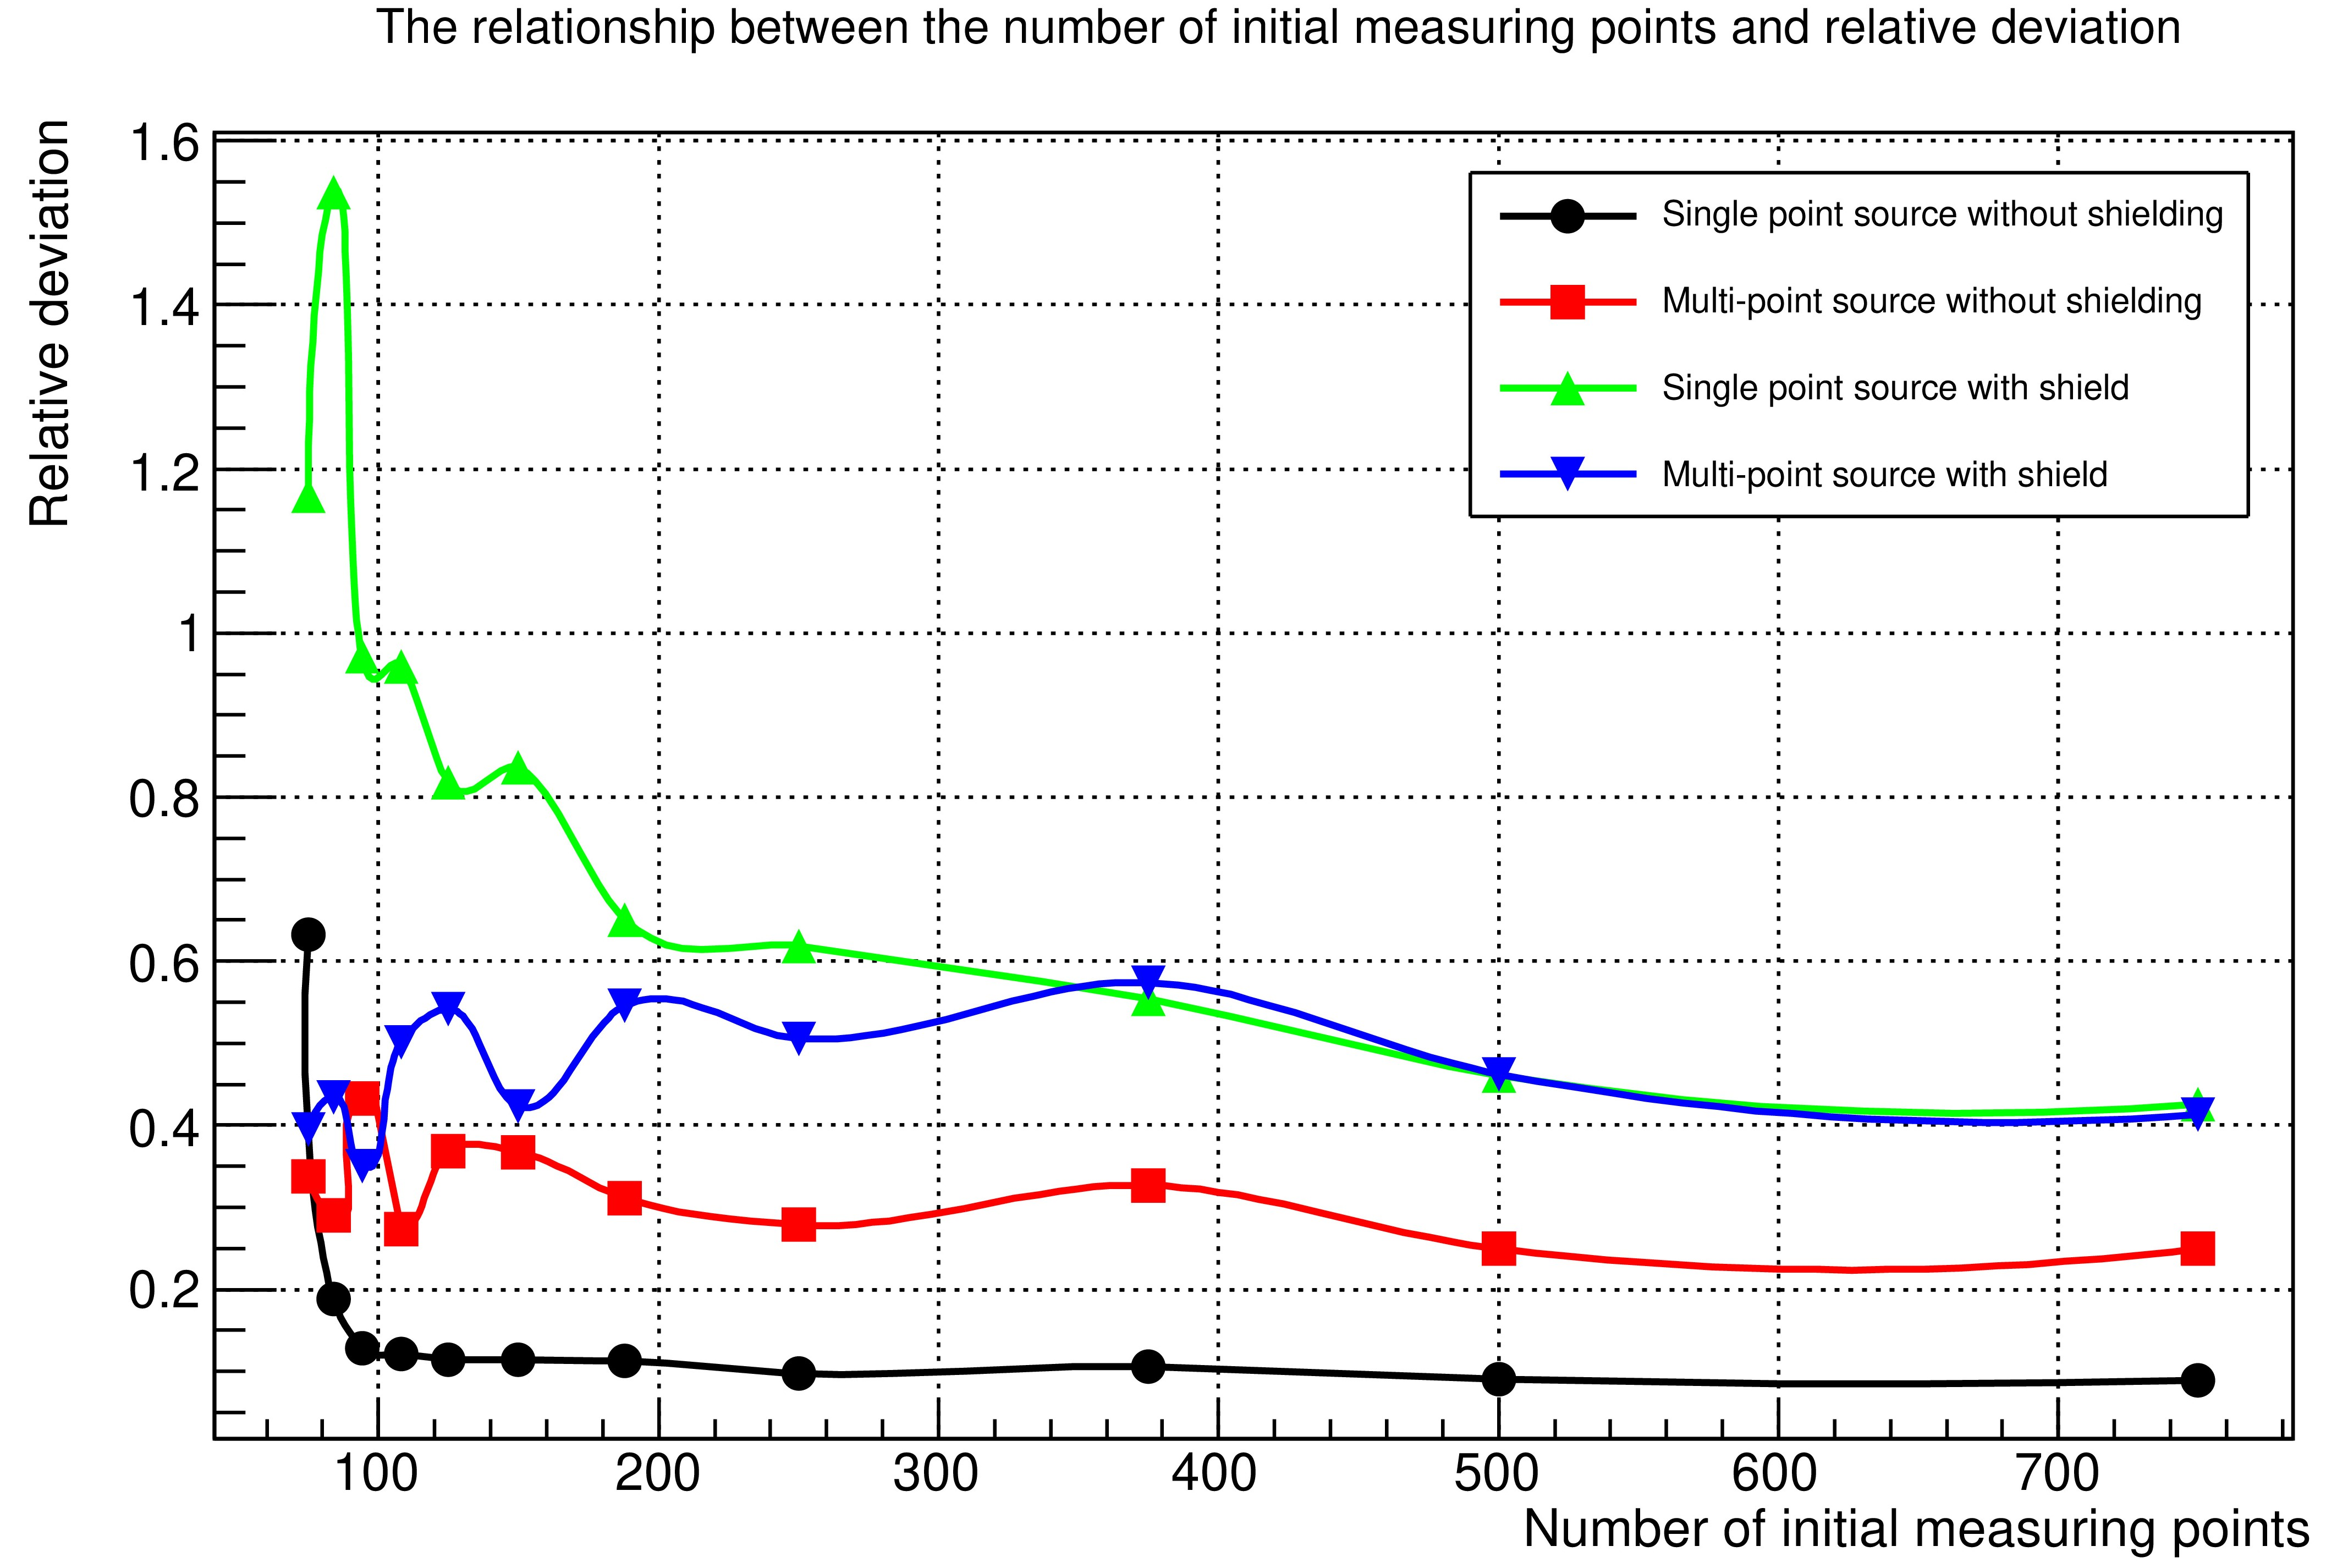
\includegraphics[width=0.8\textwidth]{figures/Deviation/MeasurePoints.jpg}
    \caption{初始测点数量与相对偏差的关系}
    \label{初始测点数量与相对偏差的关系}
\end{figure}

从图\ref{初始测点数量与相对偏差的关系}中可以看出,初始测量点数据增加时,整体相对偏差呈下降趋势。通过对不同初始测点数据进行插值重构,发现当初始测点数量较少时,通过本论文提出的插值重构算法,在插值过程中添加测点数量越多。对比四种辐射场,可以发现本论文提出的辐射场插值重构方法对无屏蔽空间辐射场重构效果较好,源项数量增加对重构相对偏差有一定影响,但相对偏差大小在一定范围内;而对带有屏蔽辐射场重构效果相对一般,主要原因是对于带有屏蔽空间辐射场,其剂量分布在屏蔽物周围变化较大,插值重构方法对变化梯度较大的数值重构效果一般。